\documentclass{sig-alternate}



\usepackage{makeidx}

%\newenvironment{titemize}{
%    \vspace{-.4\baselineskip}
%    \begin{itemize}
%    \itemsep -.1\baselineskip
%}
%{\end{itemize} \vspace{-.3\baselineskip}}
%\newcommand{\titem}{\item[$\bullet$]}
%

\usepackage{amsmath}
\usepackage{amssymb}
%\usepackage{amsthm}

\usepackage{multicol}
\usepackage{multirow}
\usepackage{graphicx}
\usepackage{color}
\usepackage{subfigure}
\usepackage{epsfig}
\usepackage{fancybox}
\usepackage{fancyvrb}

\usepackage{rotating}

\usepackage{hyperref} % comes last, as it redefines a couple of commands
\hypersetup{
    colorlinks,%
    citecolor=black,%
    filecolor=black,%
    linkcolor=black,%
    urlcolor=blue
}

\DefineVerbatimEnvironment{colorcode}%
        {Verbatim}{fontsize=\small,commandchars=\\\{\}}   % \normalsize
        %{Verbatim}{fontsize=\scriptsize,commandchars=\\\{\}}


\definecolor{DikuRed}{RGB}{130,50,32}
\newcommand{\emp}[1]{\textcolor{DikuRed}{ #1}}
\definecolor{CosGreen}{RGB}{10,100,70}
\newcommand{\emphh}[1]{\textcolor{CosGreen}{ #1}}


\newcommand{\mymath}[1]{$ #1 $}
\newcommand{\myindx}[1]{_{#1}}
\newcommand{\myindu}[1]{^{#1}}
\newcommand{\mymathbb}[1]{\mathbb{#1}}


\hyphenation{in-de-pen-dence}
\hyphenation{pa-ra-lle-lize}
\hyphenation{sub-scrip-ted}
\hyphenation{sub-scrip-ted}
\pagestyle{plain}


\begin{document}

%\conferenceinfo{ICS}{'13 Eugene, Oregon USA}


%\title{ Summarizing Accesses Without Closed-Form Solutions in Loop : Beyond Idiom Recognition }   
\title{ Summarizing Conditionally-Monotonic Subscripts}   

\numberofauthors{2}

\author{
\alignauthor
Cosmin E. Oancea\\
       \affaddr{Department of Computer Science}\\
       \affaddr{University of Copenhagen}\\
       \email{cosmin.oancea@diku.dk}
% 2nd. author
\alignauthor
Lawrence Rauchwerger\\
       \affaddr{Department of Computer Science and Eng.}\\
       \affaddr{Texas A \& M University}\\
       \email{rwerger@cs.tamu.edu}
}


\maketitle
%\thispagestyle{empty}


\pagenumbering{arabic}

\begin{abstract}

Subscripts using variables, named {\sc civ}, that cannot be expressed 
as a formula in terms of the enclosing-loop indices,  
appear in the low-level implementation of common programming abstractions 
such as filter operations or stacks or vectors in which elements are 
inserted at the end, and pose significant challenges to automatic
parallelization.

This paper presents a flow-sensitive technique that summarizes 
both {\sc civ}-based and affine subscripts to program level,
and under the same representation: Our technique (i) requires no 
modifications of the dependency test, which is agnostic to the 
original shape of the subscripts, and (ii) may prove useful
in a wider context, e.g., array {\sc ssa}. 
%, and may be applied in a wider context, e.g., array {\sc ssa}.
%
%On the one hand, our technique does not require modifications of 
%the dependency test, which is agnostic to the original shape of 
%the subscripts. 
In comparison, related work uses specialized dependency tests that 
%operate at the level of each pair of read-write subscripts, and
disambiguate each pair of read-write accesses (locally), and 
have been found less-suited than the summary-based ones in analyzing 
more complex loops. 
%than the ones based on summaries.   
%On the other hand, our technique is not restricted to 
%dependency tests and may be applied for example in the context 
%of array {\sc ssa}.
%
We report a systematic evaluation of five Fortran benchmarks that demonstrates 
  (i) efficient (scalable) parallel execution, 
 (ii) that important loops exhibiting {\sc civ} subscripts are not infrequent, and 
(iii) that our techniques covers loops that were either not reported or were 
        previously solved each with a different technique.
\end{abstract}


\category{D.1.3}{Concurrent Programming}{Parallel Programming}
\category{D.3.4}{Processors}{Compiler}


\terms{Performance, Design, Algorithms}

\keywords{
array-reference summaries, conditional induction variables}


\section{Introduction}

%%%%%%%%%%%%%%%%%%%%%%%%%%%%%%%%%%%%%%%%%%%%%%%%%%%%%%%%%%%%%%%%%%%%%%%%%%
%%% CLASSICAL ANALYSIS: Poly/Array Indexing + CIV + High-Level Contrib %%%
%%%%%%%%%%%%%%%%%%%%%%%%%%%%%%%%%%%%%%%%%%%%%%%%%%%%%%%%%%%%%%%%%%%%%%%%%%

\enlargethispage{\baselineskip}

Array-subscript analysis, e.g., array-dependence analysis~\cite{BanerjeeIneqTest,FeautrierDataflow,Pugh92theomega},
typically requires that subscript expressions are affine formulas
in the indices of the enclosing loop nest.   A known problem in 
the area of automatic loop parallelization is that a significant 
number of (important) loops exhibit subscripts 
that use induction variables that cannot be expressed by such closed-form 
formulas, because they are incremented differently, or not at all, on 
different control-flow paths of the loop.   We call such variables
{\em conditional induction variables} or {\sc civ} for short.
This paper examines parallelization of loops that exhibit 
{\sc civ} variables, which are either used for indexing or 
directly in the computation of the result.

\begin{figure}
\begin{minipage}{0.58\columnwidth}
\begin{colorcode}
k = k0     \emphh{\em Ind.}  k = k0        
DO i =1,N  \emphh{\em Var.}  DO i = 1, N      
  k = k+2    \emphh{\mymath{\Rightarrow}}    a(k0+2*i)=.. 
  a(k)=..  \emphh{\em Sub.}  ENDDO         
ENDDO            k=k0+MAX(2N,0)
\end{colorcode}
\end{minipage}
\begin{minipage}{0.35\columnwidth}
\begin{colorcode}
DO i = 1, N
 IF(cond(b(i)))THEN 
    civ = civ + 1 \emp{\mymath{\Rightarrow}{\em ?}} 
    a(civ) = ...
ENDIF ENDDO
\end{colorcode}
\end{minipage}
\hrule
\caption{Loops with affine and {\sc civ} array accesses.}
\label{fig:introEg}
\vspace{-2ex}
\end{figure}

\enlargethispage{\baselineskip}

Figure~\ref{fig:introEg} demonstrates this difficulty on a
simple example:
%
Each iteration of the leftmost loop increments variable {\tt k} by two, and
updates the element at index {\tt k} of array {\tt a}. %, i.e., {\tt a(k)}.
%
Induction-variable substitution generates the loop in the middle by replacing 
{\tt k} with the affine formula {\tt k0+2*i}, where {\tt i} is the 
loop index.   This (i) eliminates the loop-carried dependency corresponding to 
incrementing {\tt k} and (ii) enables a straightforward proof of the invariant
that two different iteration {\tt i$_1$} and {\tt i$_2$} cannot write the same
element of array {\tt a}, a.k.a., output independence: 
{\tt k0+2*i$_1$~=~k0+2*i$_2$ $\Rightarrow$ i$_1$=i$_2$}.
It follows that the middle loop can be safely parallelized.

The rightmost loop of Figure~\ref{fig:introEg} is similar to
the leftmost one, except that the increment operation and the 
array update are performed only when condition {\tt cond(b(i))} 
holds.  Since the value of {\tt civ} cannot be expressed anymore 
as a closed-form formula in {\tt i}, the previous technique would
conservatively fail to parallelize the loop, albeit this is possible.

Current solutions~\cite{Blume94RangeTest,SeqVars,PaduaStackArr,VEG,MonStmt,CohenBeyondMon} 
% Blume95symbolicrange 
use a two-step approach:
First, {\sc civ} scalars are recognized and their properties, such as 
monotonicity or cross-iteration distance, are inferred.   
Intuitively, in our example, this corresponds to determining that 
the values of {\tt civ} are (non-strictly) increasing
within the loop with step at most one.
%, which would allow, for example, 
%to compute them in parallel via a prefix-sum bulk operation. 
This paper does not contribute to this stage, but uses one 
such analysis~\cite{VEG}.

Second and more relevant, each pair of read-write subscripts is ({\em locally}) 
disambiguated, by means of {\em specialized} dependency tests that exploit
{\sc civ}'s properties and may also rely on pattern matching.
In our example, the cross-iteration monotonicity of the {\sc civ} values 
dictates that the {\sc civ} value, named {\tt civ$_2$} after increment 
in some iteration {\tt i$_2$} is strictly greater than the value,
named {\tt civ$_1$} of any previous iteration {\tt i$_1$}.
It follows by induction that the update of {\tt a(civ)}
cannot result in cross-iteration (output) dependencies, i.e.,
the system {\tt civ$_2$-civ$_1 \geq 1$} and {\tt civ$_2 = $civ$_1$}
has no solution. %, and hence, the loop can be parallelized.
Finally, the per-iteration {\sc civ} values can be (pre)computed 
via a prefix-sum parallel operation, since {\tt +} is associative.

On the other hand, summarization techniques~\cite{SUIF,LMAD,CosPLDI} aggregate 
array references across control-flow constructs, e.g., branches, loops, and  
%function calls, 
model dependency testing as an equation on the resulted abstract sets. 
In practice they have been found better suited to analyze more complex loops 
than analyses that operate at pair-of-accesses level, but they 
did not previously handle {\sc civ} subscripts.   
%
{\em This paper} presents an extension to interprocedural 
data-flow analysis that allows both affine and {\sc civ}-based subscripts 
to be effectively summarized at program level into one {\em common representation} that builds on multi-dimensional strided intervals. 
% based on {\sc lmad}~\cite{LMAD}

The gist of our technique is to aggregate symbolically the {\sc civ} 
references on every control-flow path of the analyzed loop, in terms
of the {\sc civ} values at the entry and end of each iteration or loop.
The analysis succeeds (i) if the symbolic-summary results are identical 
on all paths and (ii) if they can be aggregated across iterations %consecutive
in the interval domain. %interval domain. %as an interval.
%within our representation. % (multi-dimensional)   

For the rightmost loop of Figure~\ref{fig:introEg} we denote by 
{\tt civ$_\mu^i$} and {\tt civ$_b^i$} the values of {\tt civ} 
at the entry and end of iteration {\tt i}, respectively.
%
On the {\tt THEN} path, i.e., {\tt cond(b(i))} holds, the write set 
of array {\tt a} is interval $W_i=${\tt [civ$_\mu^i$+1,civ$_b^i$]}, 
i.e., point {\tt \{civ$_\mu^i$+1\}}, because the incremented value 
of {\tt civ} is the one live at iteration's end. 
%
On the {\tt ELSE} path, the write set of {\tt a} is the empty set, 
but is expressible with the same symbolic formula 
$W_i=${\tt [civ$_\mu^i$+1,civ$_b^i$]} under the convention 
that an empty interval has its lower bound greater than its upper bound. 
(We have used that, since {\tt civ} is not incremented, {\tt civ$_\mu^i$} 
equals {\tt civ$_b^i$}, hence {\tt civ$_\mu^i$+1$ < $civ$_b^i$}).

Aggregating $W_k$ across the first {\tt i-1} iterations results in:
$\cup_{k=1}^{i-1}W_k \ = \ ${\tt [civ$_\mu^1$+1,civ$_b^1$]~$\cup\ldots\cup$~[civ$_\mu^{i-1}$+1,civ$_b^{i-1}$]} $\ = \ $ {\tt [civ$_\mu^1$+1,civ$_\mu^i$]}, where we have used {\tt civ} values'
monotonicity and the implicit invariant {\tt civ$_b^{k-1}\equiv$civ$_\mu^{k}$},
i.e., the {\tt civ} value at an iteration end is equal to the {\tt civ}
value at the entry of the next iteration. 
%
%Since in many cases it is not possible to derive an accurate result,
%our analysis computes a pair of under/overestimate summaries, which
%are enough in practice to verify the needed invariants.
%
Finally, program invariants are modeled as abstract-set equations
that do not depend on the original shape of the subscripts, i.e., 
{\sc civ}-based or affine. 

In our example, the output independence equation:\\
$(\cup_{k=1}^{i-1}W_k)~\cap~W_i = ${\tt [civ$_\mu^1$+1,civ$_\mu^i$]}$\cap$
{\tt [civ$_\mu^i$+1,civ$_b^i$]}$ = \emptyset,~\forall \mbox{\tt{}i}$,
verifies that the write set of any iteration {\tt i} does not overlap
the write set of all previous iterations, and, by induction,
that no distinct iterations write a common element of {\tt a}.
% $\in\{\mbox{\tt{}1}..\mbox{\tt{}N}\}$,
%i.e., if the write set of any iteration {\tt i} does not overlap
%the write set of all previous iterations, then, by induction, no 
%distinct iterations write a common index of {\tt a}. 


%%The next section presents the gist of our technique on two (simplified) loops
%%from our benchmark and compares with two related approaches.  

{\bf Main contributions of the paper are:}
\begin{itemize}
    \item A flow-sensitive analysis that extends program-level 
            summarization to effectively support {\sc civ}-based 
            subscripts, 
%by meaningfully combining the control-flow 
%of the summary with the one of the {\sc civ}.
            and disambiguates loops that were not reported 
            before or were solved each with a different technique,

    \item A non-trivial code generation that separates the 
            program slice that performs the parallel-prefix-sum
            evaluation of the per-iteration {\sc civ} values 
            from the main (parallel) computation in which 
            they are plugged in,

    \item An evaluation of five difficult to parallelize benchmarks 
            with important {\sc civ}-subscripted loops, which
            shows application level speedups as high as 
            $7.1\times$ and on average $5.1\times$ on eight cores.
%            This includes all runtime overheads, 
%            e.g., {\sc civ}-values computation, which are either 
%            negligible or scale well with the degree of parallelism.

\end  {itemize}

\enlargethispage{\baselineskip}

Finally, our technique is well integrated % fully implemented and 
in a {\tt Fortran77} compiler that uses {\em hybrid analysis}, 
which verifies dataset-sensitive invariants % (statically-unverifiable)  
at runtime by evaluating a cascade of sufficient-condition 
predicates of increasing complexity, until one succeeds. 
(The cascade of predicates is statically synthesized from the summary 
equation that models the desired invariant.)
%
We note that hybrid analysis does not require modifications
but directly benefits from our technique: 

First, our analysis simplifies {\sc civ} summaries to a form 
that enables successful verification of the desired invariants. 
Second, the pre-computation of {\sc civ} values allows:
  (i) runtime verification of {\sc civ} monotonicity whenever 
          this cannot be statically established, 
 (ii) sufficient conditions for safe parallelization to 
          be expressed in terms of the {\sc civ} values at loop's 
          entry, end, and anywhere in between, and 
(iii) safe parallelization in the simple case when
        {\sc civ} are used as data, rather than for indexing,
        within the loop.
Third, summaries have a wider applicability than dependency testing,
e.g., in the context of array {\sc ssa}.


%%%%%%%%%%%%%%%%%%%%%%%%%%%%%%
%%% STRUCTURE OF THE PAPER %%%
%%%%%%%%%%%%%%%%%%%%%%%%%%%%%%

%The rest of the paper is structured as follows: Section~\ref{subsec:Background}
%provides an introduction of our overall compiler framework.
%Section~\ref{sec:Core} presents in detail our solution to extracting
%predicates that disambiguate non-linear accesses.
%Section~\ref{sec:RelWork} compares against 
%related solutions, 
%Section~\ref{sec:EmpEval} evaluates our approach on  
%a set of benchmarks rich in non-linear accesses, and
%Section~\ref{sec:Concl} concludes the paper. 



%\section{Intuition \& Background}
\section{Preliminary Concepts}
\label{subsec:Background}

\enlargethispage{\baselineskip}

Our analysis of {\sc civ} subscripts builds on four main techniques 
reported in the literature, which we have implemented 
in our compiler, but to which this paper does not claim any contributions:
%Section~\ref{subsec:Background} introduces them for completeness.
%
%Our analysis builds on the following compiler infrastructure:
First, a baseline analysis summarizes array indices into read-only~{\sc ro}, 
read-write~{\sc rw} and write-first~{\sc wf} abstract sets, using a 
representation named unified set reference ({\sc usr}).
%, which is shown in Figure~\ref{fig:USRgrammar}.
%
Second, loop independence is then modeled as an equation in the 
{\sc usr} domain. 
%
Third, whenever this equation cannot be satisfied statically, a 
predicate is extracted from it, and its evaluation verifies independence 
at runtime. 
%
Finally, the value evolution graph ({\sc veg}) is used to model the 
flow of {\sc civ} values in a loop, and to query scalars' ranges.

%, whose
%grammar is shown in Figure~\ref{fig:USRgrammar}

\vspace{1ex}
%\begin{figure}[hbt]\vspace{-1ex}
\hspace{-4ex}
\begin{tabular}{lclr}
$USR$ & ::= &  $LMAD$                 & ($n$-dim strided intervals)\\
      & {\tt~~}| & $USR \ \cup \ USR$ & (set union)\\
      & {\tt~~}| & $USR \ \cap \ USR$ & (intersection)\\
      & {\tt~~}| & $USR \ - \ USR$ & (difference)\\
      & {\tt~~}| & $Exp^{bool} \ \# \ USR$ & (gated USR)\\
      & {\tt~~}| & $_l\cup_{i=1}^{N} \ USR$ & (full recurrence)\\
      & {\tt~~}| & $_l\cup_{k=1}^{i-1} \ USR$ & (partial recurrence)\\
      & {\tt~~}| & $CallSite \ \bowtie \ USR$ & (callsite translation)
\end{tabular}%\vspace{-2ex}
%\caption{Unified Set Reference (USR) Grammar.}
%\label{fig:USRgrammar}
%\end{figure}
\vspace{1ex}

{\bf USR Construction}~\cite{HybAn}.
%
Summaries use the representation shown above %in Figure~\ref{fig:USRgrammar},
and can be seen as a {\sc dag} in which leaves correspond,
for simplicity, to strided (multi-dimensional) intervals, 
named linear memory access descriptors~\cite{LMAD} ({\sc lmad}) in the literature.
{\sc usr}'s internal nodes represent operations whose results are not
accurately representable in the {\sc lmad} domain: (i) irreducible set
operations, such as union, intersection, subtraction ($\cup$, $\cap$, $-$), 
or (ii) control flow: gates predicating
summary existence (prefixed by $\#$) or total ($_l\cup_{i=1}^N$) and partial 
($_l\cup_{k=1}^{i-1}$) unions corresponding to a loop $l$ of
index {\tt i=1,N}. 
%An example is graphically depicted in Figure~\ref{fig:USR_ROio_EXTEND_do500}.
%
We note that while {\sc usr}s are complex and accurate,
one can always under/over-estimate an {\sc usr} in the 
simpler strided-interval domain, albeit this may 
prove very conservative, i.e., $\emptyset$, or $[0,\infty]$. 
%The latter two cases are depicted in 
%Figures~\ref{fig:IndEq}~and~\ref{fig:LoopAggreg}.


{\sc usr}s are built during a bottom-up traversal of a control-flow 
reducible program.
%
In this pass, data-flow equations dictate how summaries 
are initialized at statement level, merged across branches, 
translated across call sites, composed between consecutive 
regions, and aggregated across loops. 
%
For example, the aggregation equation for a loop $l$ of index 
{\tt i=1,N} is shown in Figure~\ref{fig:LoopAggreg}:
The loop-aggregated write-first set $WF$ is obtained 
by (i) subtracting from the write-first set of iteration 
$i$, i.e., $WF_i$, the reads of any iteration preceding $i$,
and (ii) by uniting the per iteration sets. %these results for all $i=1..N$.

\begin{figure}[t]
%\hrule ~
	\begin{tabular}{l r} \hspace{-5ex} 
	\multirow{2}{*}[22.5ex]
    {
   	  \subfigure[$\mbox{~~~~~~~~~~~~~~~~~~~~~}$]{ % Loop-Aggregation Equations
          \label{fig:LoopAggreg} 
		\makebox[0.4\textwidth][l] { \vbox{\scriptsize
SUMMARIZE($REG_i$, $i = 1, N$) \vspace{1ex} \newline
$\mbox{ }(WF_i, RO_i, RW_i) \leftarrow REG_i$ \vspace{1ex} \newline
$\mbox{ }R_i = RO_i \cup RW_i$ \vspace{2ex} \newline
$\mbox{ }WF = \bigcup_{i=1}^{N} (WF_i - \bigcup_{k=1}^{i-1}R_k)$ \vspace{1ex} \newline
%$\mbox{~~~~~~~~~~~~~~~~~~}\bigcup_{k=1}^{i-1}R_k)$ \vspace{1ex} \newline
$\mbox{ }RO = \bigcup_{i=1}^{N} RO_i - $ \newline %\bigcup_{i=1}^{N}(WF_i \cup RW_i)$ \vspace{1ex} \newline
$\mbox{~~~~~~~~~}\bigcup_{i=1}^{N}(WF_i \cup RW_i)$ \vspace{1ex} \newline
$\mbox{ }RW = (\bigcup_{i=1}^{N} R_i) - (WF \cup RO)$ \vspace{1ex} \newline
$\mbox{ }$RETURN $(WF, RO, RW)$ \vspace{1ex}
}
		}          			
	  } 
	} & { \hspace{-27ex}
	  \subfigure[$\mbox{~~~~~~~~~~~~~~~~~~~~~~~~~~~~~~~~~~~~~~~~~~~~~~~~~~~~~~}$]{ %Independence Equations
          \label{fig:IndEq} 
		\makebox[0.57\textwidth][l] { \vbox{\scriptsize
OUTPUT INDEPENDENCE EQ:\vspace{1ex} \newline
$\mbox{ }\{ \cup_{i=1}^{N}(WF_i \cap (\cup_{k=1}^{i-1}WF_k))\} = \emptyset$ \vspace{4ex} \newline
FLOW/ANTI INDEPENDEP EQ:\vspace{1ex} \newline
$\mbox{ }\{(\cup_{i=1}^{N}WF_i) \cap (\cup_{i=1}^{N}RO_i)\} \mbox{ }\cup\mbox{ }$ \vspace{1ex} \newline
$\mbox{ }\{(\cup_{i=1}^{N}WF_i) \cap (\cup_{i=1}^{N}RW_i)\} \mbox{ }\cup\mbox{ }$ \vspace{1ex} \newline
$\mbox{ }\{(\cup_{i=1}^{N}RO_i) \cap (\cup_{i=1}^{N}RW_i)\} \mbox{ }\cup\mbox{ }$ \vspace{1ex} \newline
$\mbox{ }\{ \cup_{i=1}^{N}(RW_i \cap (\cup_{k=1}^{i-1}RW_k))\}=\emptyset$ \newline
%$\mbox{~~~~~~~~~~~~~~~~}=\emptyset$ \vspace{1ex}
}
		}
	  } 
	} 
\end{tabular}
\hrule
\caption{ (a) Summarizing Across a Loop and (b) Modeling Loop Independence with Set Equations.}
\label{fig:UsrEq} %
\end{figure}

\vspace{1ex}

{\bf Independence Equations}. Figure~\ref{fig:IndEq} shows the {\sc usr}
equations, of form $S=\emptyset$, that model loop independence. 
The output independence equation
states that if for any $i$, the write-first set of iteration $i$
does not overlap with the write-first set of any iteration preceding
$i$, then, by induction, no two  iterations write the same % different
location. Similarly, for flow/anti independence it is checked 
(i) the disjointness of the total unions of the per-iteration {\sc wf}, 
{\sc ro}, and {\sc rw} set, and (ii) that the {\sc rw} sets of any two 
iterations do not overlap.

\vspace{1ex}

{\bf Synthesizing Independence Predicates}~\cite{CosPLDI}. %~\cite{SummaryMonot,CosPLDI}.  
When the independence equation
is not statically satisfied, we use a translation scheme $\mathcal{F}$,
from the {\sc usr} language to a language of % expressive
predicates, named {\sc pdag}, to extract a sufficient-independence condition: 
$\mathcal{F} : $ {\sc usr} $\rightarrow$ {\sc pdag},  
$\mathcal{F}(S) \Rightarrow S = \emptyset$. The result is then separated
into a cascade of predicates that are tested at runtime in the order of 
their complexities.  
If output dependencies cannot be disproved then privatisation is
necessary. If $WF_i$ is loop invariant then only the last iteration 
writes to non-private storage (static last value).

\vspace{1ex}

{\bf Value-Evolution Graph}~\cite{VEG} ({\sc veg}) is a {\sc dag}  %~\cite{VEG}
that represents the flow of values between gated-{\sc ssa}~\cite{GatedSSA} names 
of a scalar variable.  
%
{\sc veg}s are constructed on demand at loop and subroutine levels.
%
The entry node, e.g., merging cross-iteration values,  is named 
the $\mu$ node and is drawn via a double circle. The recurrence is 
depicted via a dotted line, named the {\em back edge}, and the
back node is drawn in a hexagon.
%
Regular nodes, drawn in circles, correspond to reduction-like statements.
For example Figures~\ref{fig:VegACTFOR}~and~\ref{fig:VegCORREC} 
depict the {\sc veg}s for the running-example loops in 
Figure~\ref{fig:codeActforCorrec}, which will be discussed later. 
Even without looking at the code, one can tell that both loops
have a variable named {\tt civ} that is incremented on some loop
paths with exactly {\tt 1} and {\tt 3*C(i)}, respectivelly, 
and is not updated on other paths. 
%e.g., {\tt civ@3 = civ@2 + 1} is summarized via the edge 
%of evolution $1$ between {\tt civ@2} and {\tt civ@3} in Figure~\ref{fig:VegACTFOR}.
%

Note that branch conditions are not explicit in the {\sc veg}, 
but they are easily found from the gated-{\sc ssa} definition 
of $\gamma$-merged {\sc civ}s. % node ($\gamma$) . 
%
Nodes corresponding to arbitrary assignments, i.e., not a reduction, are
named input nodes and are drawn in rectangles. 
%
A conditional induction variable ({\sc civ}) corresponds to a
particular {\sc veg}, in which:
  (i) the $\mu$ node is unique, dominates all other {\sc veg} nodes,
            i.e., is reachable from within the {\sc veg} only through its
            unique back edge, %on path that do not pass through other $\mu$ nodes,
%
 (ii) no node in the associated {\sc veg} can be reached via any input nodes, and 
%
(iii) the $\mu$-node values are provably monotonic.
            %i.e., on all {\sc veg}'s paths.
            
Both {\sc veg} examples comply with these rules.
For example, the {\tt 3*C(i)} evolution in 
Figure~\ref{fig:VegCORREC} is proven positive at the 
point of use, because path 
${\tt civ@2}\rightarrow{\tt civ@3}\rightarrow{\tt civ@4}$
is guarded by condition {\tt C(i).GT.0} (as per the 
gated-{\sc ssa} definition of $\gamma$-node {\tt civ@4}).
If this is not possible statically, analysis speculatively
assumes monotonicity, and verifies it at runtime in the slice 
that (pre)computes the {\sc civ} values. 


\section{Summarizing Monotonic CIVs}
\label{sec:MonotonicCiv}

%The introductory example showed a relatively straightforward
%analysis that inferred an {\em accurate} summary for a loop 
%exhibiting {\em only} {\sc civ}-based subscripts.   
The introductory example showed a simple loop exhibiting 
{\em only} (one) {\sc civ}-based subscripts that could be
{\em accurately} summarized.
%
In practice however, important loops use {\em both} %(benchmark) 
affine and {\sc civ}-based subscripts on the same array, hence 
terms of both kinds may appear in the set expression %formula 
of the accurate summary, which cannot be simplified
to an interval.
%and an exact interval-based
%summary may not even exist, regardless.

Our analysis is implemented as an extension of baseline 
summarization for the special cases of loop and iteration 
aggregation (and callsite translation), because at these 
levels the {\sc civ}-value properties, summarized by 
{\sc veg}, can be effectively used.
%
To compute the symbolic summary across all paths, the analysis
needs to combine the control-flow of the summary, e.g., 
encoded in {\sc usr}'s gates, with the control flow of the {\sc veg}. 
The key idea here is to conservatively project the summary terms 
on the {\sc veg} and to merge across all {\sc veg} paths.
It follows that our analysis computes under and overestimate
summaries, but accuracy is recovered whenever the under and 
overestimate are identical.
%which also allows separate aggregation of the affine 
%and {\sc civ}-based terms (of different {\sc civ} variables). 
%
%
Over/under-estimation also allows (separate) aggregation of the 
affine and {\sc civ}-based subscripts, which are typically
accurate enough to verify the desired invariant.
%In these cases extending analysis to cover {\em under/over-estimates}
%allows separate aggregation of the two kinds of subscripts,
%while still verifying the desired invariant. 
%Furthermore, if the over and under-estimate are identical,
%the summary is accurate, and underestimates may be used to 
%simplify other exact summaries, e.g., the write-first summary
%may be used to filter out terms of the read-write summary. 
%

Discussion is organized as follows:
Section~\ref{Intro:RelAppLim} intuitively demonstrates our approach 
on two running-example loops. %from the \textsc{Perfect-Club} suite.
%
{\em Section~\ref{subsec:ProblemHL}} establishes a uniform notation and
states the problem at a high level.
%
{\em Section~\ref{subsec:BasicTechn}} presents the basic flow-sensitive 
analysis technique for summarizing over and underestimates, and 
demonstrates it on the examples depicted in 
Figure~\ref{fig:codeActforCorrec}.
%
{\em Section~\ref{subsec:Track}} shows several enhancements
to the basic technique that solve %allow automatic parallelization of %   
more difficult loops, such as {\tt EXTEND\_do400} from benchmark {\sc track}.
%
For example, the read-only (accurate) {\sc usr} in Figure~\ref{fig:Track}
can be simplified to point {\tt \{i-1\}} by filtering out the terms
that belong to the write-first underestimate.
%Section~\ref{subsec:Track}.
%
Finally, {\em Section~\ref{subsect:CivImplem}} details on the overall 
implementation, and focuses on how to (pre)compute safely and in parallel 
the {\sc civ}$_\mu$ values associated to each iteration.


\subsection{Demonstration on Two Code Examples}
\label{Intro:RelAppLim}

Figure~\ref{fig:codeActforCorrec} depicts two loops
using both {\sc civ} and affine subscripts, where the {\tt civ} variable 
is written in (gated) single-static-assignment ({\sc ssa}) notation~\cite{GatedSSA}.
%
For example, the statement {\tt civ@2=$\gamma$(i.EQ.1,civ@1,civ@4)}
has the semantics that the fresh variable {\tt civ@2} takes, depending 
on the evaluation of {\tt i.EQ.1}, either the value 
of {\tt civ@1} for the first iteration, or the value of 
{\tt civ@4} for all other iterations.

\enlargethispage{\baselineskip}

One difficulty in parallelizing loop {\tt ACTFOR\_do240} is to
prove that array {\tt X} can be privatized, i.e., that all
indices of {\tt X} which are read in the second inner loop have been 
written in the first inner loop by the same iteration of the outer loop.
The plan is to {\em summarize} the read and written indices at the level of
the first and second inner loops, respectively, and to prove that an
overestimate of the read set  is included in an underestimate 
of the write set (of indices) of the same outer-loop iteration {\tt i},
i.e., $\lceil R_i\rceil \subseteq \lfloor W_i\rfloor$.
%
The summarization analysis is similar to the one used in the introductory 
example, except that here we use the convention % and in the rest of the paper  
that array indices start from {\tt 0} rather than {\tt 1}.
The read subscripts correspond to the affine access {\tt X(j)}, where
the loop index {\tt j} ranges in {\tt 1..civ@5},
hence $\lceil R_i\rceil = ${\tt[0,civ@5-1]}.

\begin{figure}
\begin{minipage}{0.45\columnwidth}
\begin{colorcode}
DO i = 2, N, 1
 civ@1 = 0
 DO j = 1, i-1, 1
  civ@2=\mymath{\gamma}(civ@1,civ@4)
  IF IA(j) .NE. 0 THEN
   civ@3 = 1 + civ@2
   {\bf{}X}(civ@3) = j
  ENDIF
  civ@4=\mymath{\gamma}(civ@3,civ@2)
 ENDDO
 civ@5=\mymath{\gamma}(civ@4,civ@1)
 IF civ@5 .NE. 0 THEN
  DO j = 1, civ@5
   sum = sum+Z( {\bf{}X}(j) )
ENDDO ENDIF ENDDO
\end{colorcode}
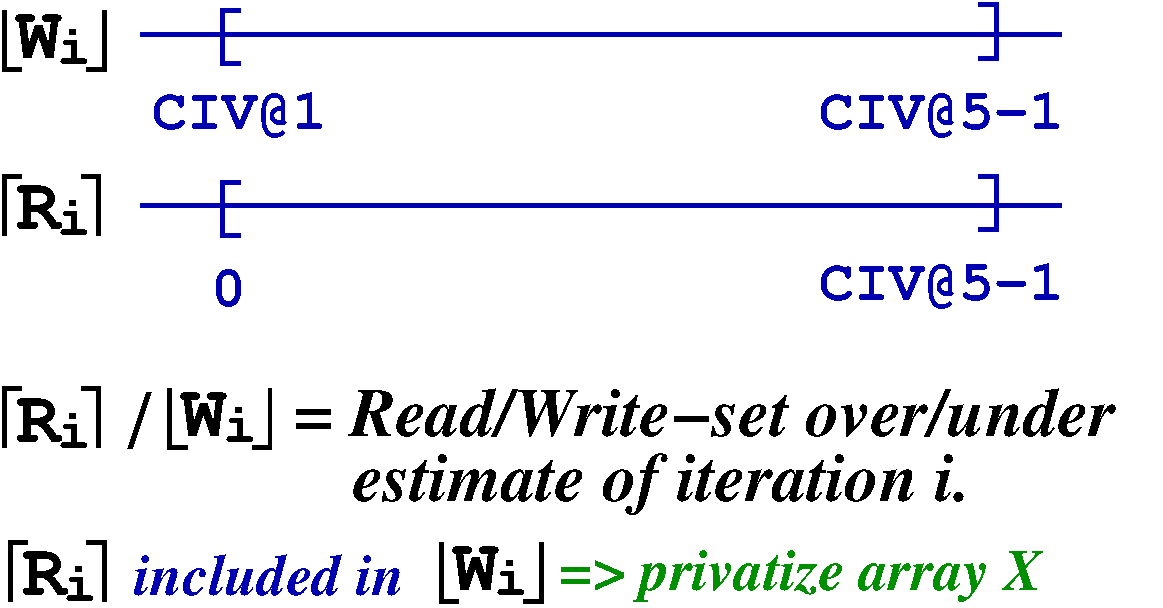
\includegraphics[width=1.1\textwidth]{Figures/ActforRWsets} 
\end{minipage}
\begin{minipage}{0.48\columnwidth}
\begin{colorcode}
civ@1 = Q
DO i = M, N, 1
 civ@2=\mymath{\gamma}(civ@1,civ@4)
 .. = {\bf X}(i) ..
 IF C(i) .GT. 0 THEN
  DO j = 1, C(i), 1
   IF(..){\bf{}X}(j+civ@2       )=..
   IF(..){\bf{}X}(j+civ@2+  C(i))=..
   IF(..){\bf{}X}(j+civ@2+2*C(i))=..
  ENDDO
  civ@3 = 3 * C(i) + civ@2
 ENDIF
 civ@4=\mymath{\gamma}(civ@3,civ@2)
ENDDO
civ@5=\mymath{\gamma}(civ@4,civ@1)  
\end{colorcode}
\hspace{2ex}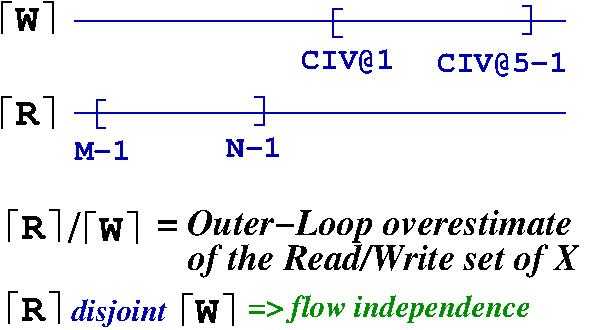
\includegraphics[width=1\textwidth]{Figures/CorrecRWsets} 
\end{minipage}
\hrule
\caption{(a) {\tt ACTFOR\_do240} and (b) {\tt CORREC\_do401} simplified loops 
            from {\sc bdna} bench, {\sc Perfect-Club} suite.}
\label{fig:codeActforCorrec}
%\vspace{-1.5ex}
\end{figure}
%   \label{fig:CodeACTFOR}     \label{fig:CodeCORREC} 



%, where we use the 
%convention that array indexing starts from {\tt 0} rather than {\tt 1}.
%
The written subscripts correspond to the {\sc civ} access {\tt X(civ@3)}, %-based
and are summarized for an iteration of the first-inner loop as
interval  {\tt[civ@2,civ@4-1]}, i.e., using the {\sc civ} values at 
the beginning and end of an iteration.
%\footnote{Formula also holds 
%for the {\tt ELSE} branch of {\tt IF(IA(j).NE.0)} under the convention 
%that {\tt lb $>$ ub} $\Rightarrow$ {\tt [lb, ub]}$\ \equiv \ \emptyset$.}:
This is satisfied on the {\tt THEN} branch because element {\tt civ@3-1}
is written and the {\sc civ} subscript is incremented, i.e., 
{\tt civ@4=civ@3=civ@2+1}. It also holds on the {\tt ELSE} branch
which neither increments {\sc civ} nor writes anything under the convention 
that an empty interval has its lower bound greater than its upper bound,
i.e., {\tt civ@2=civ@4>civ@4-1}.
%
%This holds on the {\tt THEN}
%which increments the {\sc civ} subscript because {\tt civ@4=civ@3=civ@2+1},
%and also on the {\tt ELSE} branch under the assumption..
%
Since the iteration summary is identical on all paths the underestimate 
set of written indices for the (first inner) loop is obtained by suitably 
replacing {\tt civ@2} and {\tt civ@4} with the lower and upper bounds of 
their ranges, i.e., {\tt civ@1} and {\tt civ@5}, which results in 
$\lfloor W_i\rfloor={\tt [0,civ@5-1]}$.
(This is similar to aggregating across a loop whose index ranges 
    from {\tt{}civ@1=0} to {\tt{}civ@5-1}, because the {\tt civ} 
    values are monotonic with step at most {\tt 1}.)

Finally, the computed read and write over and under-estimates are identical 
for any outermost iteration {\tt i}, hence the desired invariant 
$\lceil R_i\rceil \subseteq \lfloor W_i\rfloor$ holds, and array {\tt X} 
can be safely privatized. 
%
Furthermore, since an outer iteration uses the values of {\tt X} that 
have been produced in the same iteration, range analysis determines that 
the value {\tt X(j) $\in$ [1,i-1]}, because the update 
{\tt X(civ@3)=j} occurs in the first inner loop of index {\tt j $\in$ [1,i-1]}. 
%
This information allows to similarly prove privatization 
of {\tt Z} (the writes to {\tt Z} not shown).
%
Outer-loop parallelization is thus safe because 
privatization has eliminated all carried dependencies on {\tt X} and {\tt Y}. %and {\tt Z}.

\vspace{1ex}
Parallelizing loop {\tt CORREC\_do401} in Figure~\ref{fig:codeActforCorrec}(b) 
requires more work: one needs to prove that the outer-loop's read and write 
sets of {\tt X} do not overlap, and also that the write sets of  
different iterations do not overlap, i.e., flow and output independence. 
Array {\tt X} is read on index {\tt i}, which ranges from {\tt M} to {\tt N},
hence the read(-only) overestimate across the loop is 
{\tt$\lceil R \rceil =\cup_{i=M}^{N}(i-1)=$[M-1,N-1]}.
%since the loop bounds are {\tt M} and {\tt N}.


Computation of the write-set {\em overestimate} across the inner loop 
(i)  conservatively assumes that the {\tt if} branches are always taken, and
(ii) summarizes the three affine loop updates 
to interval {\tt[civ@2,civ@2+3*C(i)-1]},
e.g., {\tt X(j+civ@2)} generates {\tt[civ@2,civ@2+C(i)-1]}, since  
{\tt j$\in$\{1$\ldots$C(i)\}}.

Similar to the introductory example, outer-loop aggregation
analyzes each path of an iteration:
On the path on which {\tt C(i).GT.0}, we have %that 
{\tt civ@4$=$civ@3$=$civ@2+3*C(i)}, and the path summary is
rewritten as {\tt [civ@2,civ@4-1]}. The other path neither 
updates {\tt X} nor increments {\tt civ}, hence it accepts the
same summary {\tt[civ@2,civ@4-1]$=\emptyset$}.
%, since the lower bound is greater than the upper bound.

Since {\tt civ} is updated only when {\tt C(i)} is positive,
its values are monotonically increasing within the loop with
the lower and upper bounds being {\tt civ@1=Q} and {\tt civ@5}. 
It follows that the write-set overestimate of the outer loop is 
interval $\lceil W \rceil = \lceil \cup_{i=M}^{N}W_i\rceil =${\tt[Q,civ@5-1]}.
Flow independence requires   
$\lceil W\rceil\cap\lceil R \rceil \equiv {\tt [M-1,N-1]}\cap{\tt{}[Q,civ@5-1]}=\emptyset$,
and a sufficient condition for this equation to hold is (easily) extracted:
${\tt Q} \ge {\tt N}~\vee~{\tt M} > {\tt{}civ@5}$.
%
Finally, output independence is proven statically, similarly to the 
{\sc civ} loop of Figure~\ref{fig:introEg}.
%statically in a fashion similar 
%to the one shown for the {\sc civ} loop in Figure~\ref{fig:introEg}.
%in a similar fashion, i.e., 
%it is modeled via a set equation whose terms are computed as before.

\vspace{1ex}
We conclude this section with {\em two high-level observations}: %  
{\em First}, our analysis summarizes {\sc civ} and affine subscripts
much in the same way, and enables a dependence test which is agnostic
to the kind of subscripts that were used.
%
%is driven by verifying the algebraic 
%invariants that allow the {\sc civ} subscripts to be summarized 
%via the same symbolic set on all control-flow paths:
%In both examples (i) {\sc civ} (and affine) subscripts are 
%summarized much in the same way, and (ii) the dependence %/privatization 
%test is agnostic to the kind of subscripts that were used.
%operate uniformly on summaries
%obtained from regular and {\sc civ} accesses.
% 
%the resulted summaries
%and succeed without any other modifications or pattern-matching support. 
%
These properties do not seem to hold for related solutions: For example, 
a technique~\cite{CohenBeyondMon} that disambiguates pairs of accesses 
of shape {\tt \{X(civ),X(civ+CT)\}} may prove the output 
independence of {\tt CORREC\_do401}, but will not prove the flow-independence 
of either loop.
Similarly, pattern-matching the consecutively-written single-index-array
access~\cite{PaduaStackArr,VEG} solves loop  {\tt ACTFOR\_do240} but not
{\tt CORREC\_do401}.


{\em Second}, summary approximation has been key to successful
analysis. With the second code, overestimating the write set 
of the inner loop by assuming that all branches are taken 
allowed the {\sc civ} subscripts to be aggregated in the 
interval domain. 
More importantly, note that the separation of the 
read and write sets cannot be verified statically, i.e.,
flow independence requires a runtime condition. 
It follows that the accurate write-first\footnote{
For simplicity, the discussion used read/write sets, 
but our analysis computes read-only, read-write and write-first sets.
}
({\sc wf}) summary at the (outer) iteration level is the 
set-difference between the terms corresponding to the inner-loop 
{\sc civ}-aggregated subscripts and the affine (read) subscript {\tt i},
respectively.  While the accurate {\sc wf} summary cannot be aggregated 
as an interval across the outer loop, its overestimate,
which includes only the {\sc civ} term, can and is sufficient
for testing loop independence. Furthermore, if an affine 
(or different-{\sc civ})
write access is added to the code, the {\sc wf} overestimate
is still computable by separately aggregating the two
terms and uniting the results.%taking the union of the results.

\subsection{Notations and Problem Statement}
\label{subsec:ProblemHL}

We denote by $\mathcal{L}$ a normalized loop of index $i\in\{1..N\}$ that
exhibits subscripts using {\sc civ} variables, which were defined
in Section~\ref{subsec:Background}. %, and denote such a variable by {\tt {\it CIV}}.
%
We denote by $U_i$ one of the write-first ({\sc wf}), read-write ({\sc rw})
or read-only ({\sc ro}) set-expression summaries of some array {\tt X} 
corresponding to iteration $i$ of loop $\mathcal{L}$, where the {\sc usr}'s 
leaves, i.e., {\sc lmad}s, may use {\sc civ} variables. 
%
For simplicity, we consider {\sc lmad}s to be 
strided intervals, i.e., $[l,u]^s=\{l, l+s, l+2*s, .., u\}$.
If $s=1$, we omit writing $s$; if the interval 
is point $p$, we write it $\{p\}$.
  

The addressed problem is to compute symbolic under/over-estimates in the 
interval domain, denoted by $\lfloor A \rfloor$/$\lceil A \rceil$, 
for $U = \cup_{i=1}^{N} U_i$.
%
In the same way in which loop aggregation of an affine subscript  
eliminates the loop index $i$ from the result summary,
we declare {\sc civ}-{\em aggregation} across $\mathcal{L}$ {\em successful} 
if $\lfloor A \rfloor$ ($\lceil A \rceil$) does not depend on any loop-variant
symbols, e.g., any symbol in {\tt CIV}$_{\mu}$'s  {\sc veg}. %associated

For example, in Figure~\ref{fig:codeActforCorrec}(a), the affine
subscript of {\tt X(j)}, expressed as {\tt\{j-1\}}, is aggregated across 
the second inner loop as {\tt[0,civ@5-1]}, which is independent on {\tt i}. 
Similarly, we would like to summarize the {\sc civ} access
{\tt X(civ@3)}, expressed as {\tt\{civ@3-1\}}, across 
the first inner loop as interval {\tt[0,civ@5-1]}. 
%
In essence this would allow to treat {\em uniformly} and {\em compositionally} 
{\sc civ}-based and affine summaries, e.g., the compiler can now prove that $X$ 
is privatizable in the outer loop since the read set is covered by the write-first 
set of the same iteration. 
Furthermore, the output of a {\sc civ}-summarized loop may 
become the input for {\sc civ}-based summarization of an outer loop,
e.g., the difficult loops {\tt EXTEND\_do500} and {\tt \_do400}
from {\tt track} benchmark.


%
Examining the terms appearing in the loop-aggregation and independence 
equations of Figure~\ref{fig:UsrEq}, we observe that we also need to similarly
reshape per-iteration ($U_i$) and partial-recurrence summaries 
($\cup_{k=1}^{i-1} U_k$), 
denoted by $A_i$ and $A_{k=1}^{i-1}$, respectively. 
%
Successful reshaping of $U_i$ means that $A_i$
depends only on the $\mu$ node, {\tt CIV}$_{\mu}^{i}$, 
and the back node, {\tt CIV}$_{b}^{i}$, of iteration $i$.
For $\cup_{k=1}^{i-1} U_k$ it means that $A_{k=1}^{i-1}$ depends
only on the {\tt CIV}$_{b}^{i-1}$ value of iteration $i-1$, which is
equal with the  {\tt CIV}$_{\mu}^{i}$ value of iteration $i$.
This allows to replace {\tt CIV}$_b^{i-1}$ with {\tt CIV}$_{\mu}^i$ in
$A_{k=1}^{i-1}$, and, as such, to compare $WF_i$ and $\cup_{k=1}^{i-1} WF_k$, 
e.g., an empty intersection implies output independence. 
%e.g., to prove that their intersection is empty, hence to establish %loop's 
%output independence.
%

\subsection{Basic Flow-Sensitive-Analysis Techinque}
\label{subsec:BasicTechn}

\begin{figure}[t]
\begin{small}
({\sc lmad},{\sc lmad},{\sc lmad}) {\bf CIVSUM}($U_i :$~{\sc{}usr}) {\bf raises Exception Fail}\vspace{1ex} \newline
$\mbox{ }\mbox{ }$// {\bf {\em Output:}} 
($A_i \equiv U_i$, $A \equiv \cup_{i=1}^{N} U_i$, $A_{k=1}^{i-1} \equiv \cup_{k=1}^{i-1} U_i$) or {\bf Fail}s. \vspace{2ex} \newline
$\mbox{ }\mbox{ }${\bf1.} \textsc{Over/Under-estimate $U_i$ by a union of gated intervals}\vspace{1ex} \newline
$\mbox{ }\mbox{ }\mbox{ }\mbox{ }\mbox{ }\mbox{ }\mbox{ }$ $(g_1\#L_1) \cup ... \cup (g_m\#L_m)\leftarrow U_i$: \vspace{2ex} \newline
$\mbox{ }\mbox{ }${\bf2.} \textsc{Project each} $L_k, k\in\{1..m\}$, \textsc{on a VEG node} {\tt CIV@q}, \vspace{1ex} \newline
$\mbox{ }\mbox{ }\mbox{ }\mbox{ }\mbox{ }\mbox{ }\mbox{ }\mbox{ }$
            \textsc{which is the civ-immediate (post) dominator of} \vspace{1ex} \newline 
$\mbox{ }\mbox{ }\mbox{ }\mbox{ }\mbox{ }\mbox{ }\mbox{ }\mbox{ }$
            \textsc{the program point where} $L_k$ \textsc{was summarized} \vspace{2ex} \newline 
$\mbox{ }\mbox{ }${\bf3.} {\bf For Each} \textsc{VEG path, symbolically unite (exactly) the}\vspace{1ex} \newline 
$\mbox{ }\mbox{ }\mbox{ }\mbox{ }\mbox{ }\mbox{ }\mbox{ }\mbox{ }$
            \textsc{$L_k$'s on that path into one interval $L_{path}$.}\vspace{1.5ex}\newline 
$\mbox{ }\mbox{ }\mbox{ }\mbox{ }\mbox{ }\mbox{ }\mbox{ }\mbox{ }$
            {\bf If} $L_{path}$ \textsc{cannot be written in terms of the} {\tt CIV$_\mu$} {\sc and} 
$\mbox{ }\mbox{ }\mbox{ }\mbox{ }\mbox{ }\mbox{ }\mbox{ }\mbox{ }$
            {\tt CIV$_b$} {\sc nodes} {\bf Then raise Fail}.\vspace{1.5ex} \newline
$\mbox{ }\mbox{ }\mbox{ }\mbox{ }\mbox{ }\mbox{ }\mbox{ }\mbox{ }$
            {\bf If} \textsc{in underestimate case} {\bf Then} \textsc{check that the condi-}
$\mbox{ }\mbox{ }\mbox{ }\mbox{ }\mbox{ }\mbox{ }\mbox{ }\mbox{ }\mbox{ }\mbox{ }\mbox{ }$
\textsc{tion of the VEG-$path$ implies $g_k$}. {\bf Else} $L_k \not\in path$.\vspace{2ex}\newline
$\mbox{ }\mbox{ }${\bf4.} {\bf If} \textsc{all $path$s have identical $L_{path}$} {\bf Then} $A_i = L_{path}$, \textsc{and}\vspace{1ex}\newline 
$\mbox{ }\mbox{ }\mbox{ }\mbox{ }\mbox{ }\mbox{ }\mbox{ }\mbox{ }\mbox{ }$
            \textsc{$A$ and $A_{k=1}^{i-1}$ are computed by exploiting the monoto-}\vspace{1ex}\newline 
$\mbox{ }\mbox{ }\mbox{ }\mbox{ }\mbox{ }\mbox{ }\mbox{ }\mbox{ }\mbox{ }$
\textsc{nicity and the symbolic bounds of {\tt CIV$_\mu$} {\sc and} {\tt CIV$_b$}.}\vspace{1ex}\newline
$\mbox{ }\mbox{ }\mbox{ }\mbox{ }\mbox{ }\mbox{ }\mbox{ }\mbox{ }\mbox{ }$ {\bf Else raise Fail.}\vspace{1ex}
\end{small}
\hrule
\caption{ CIV-Based-Summarization Pseudocode.}
\label{fig:BasicTechnique} %
\end{figure}


The algorithm that implements the basic analysis is depicted in 
Figure~\ref{fig:BasicTechnique} and has four main stages: 
%The basic analysis consists of four main stages: 
{\em First}, under and overestimates of $U_i$ are computed under the form 
of a union of gated-interval pairs.   %{\sc lmad}s
{\em Second}, the intervals that use {\sc civ} variables are 
associated with a {\sc civ} node on the corresponding {\sc veg} graph.
{\em Third}, each {\sc veg} path is summarized via an interval expressed 
in terms of the {\tt CIV$_\mu$} and {\tt CIV$_b$} nodes. 
{\em Finally}, path intervals are merged across all paths, according to 
the under/over-estimate semantics, to yield the iteration-level interval $A_i$.
Total and partial-recurrence intervals, $A$ and $A_{k=1}^{i-1}$, 
are computed by suitably substituting {\tt CIV$_\mu$} and 
{\tt CIV$_b$} in $A_i$ with suitable ({\sc veg}) bounds,
which is safe due to the cross-iteration monotonicity of {\sc civ} values.
The remaining of this section details and demonstrates each algorithmic stage
on the loops presented in Figure~\ref{fig:codeActforCorrec}.

%\newcounter{taskCnt}
%\setcounter{taskCnt}{0}
%\newcommand{\nexttask}{\addtocounter{taskCnt}{1}\arabic{taskCnt}}
%
%\paragraph{\nexttask. USR Splitting} 
%

\vspace{1ex}

{\bf 1. USR Splitting.}
Due to space constraints, we do not present here
the algorithm used to decompose an {\sc usr} into a union of 
gated-interval ${\tt g}\#L$ pairs, where $L$ is an interval and 
{\tt g} is a condition predicating $L$'s existence.  
We just note that it is always possible to build an interval
under/overestimate of an {\sc usr}, via a recursive pattern-matching of 
the {\sc usr}'s shape~\cite{SummaryMonot}, and enhancing the algorithm to 
also gather the gate information does not pose any significant challenges.   

For example, with the (first inner) loop of index {\tt j} in Figure~\ref{fig:codeActforCorrec}(a), 
the $WF_j$ summary of array {\tt X} is already in gated-interval form, i.e., 
${\tt (IA(j).NE.0)}\#\{{\tt civ@3-1}\}$,
hence the over and underestimates of $WF_j$ are identical. 

With the loop in Figure~\ref{fig:codeActforCorrec}(b), the 
write-first underestimate $\lfloor WF_i\rfloor$ of array {\tt X} 
is the empty set, because {\tt X} is (only) conditionally updated in 
the inner loop, and the gated overestimate is  
$\lceil WF_i\rceil={\tt{}(C(i).GT.0)}\#[{\tt civ@2, civ@2+3*C(i)-1}]$.
%due to the guarded write accesses in the loop of index {\tt j}.


\begin{figure}[t]
	\begin{tabular}{lr} \hspace{-5ex} % @{\hspace{0.15\textwidth}}
	\multirow{2}{*}[40ex] 
    {  
			\subfigure[Loop {\tt ACTFOR\_do240}.]{
          			\label{fig:VegACTFOR} 
          			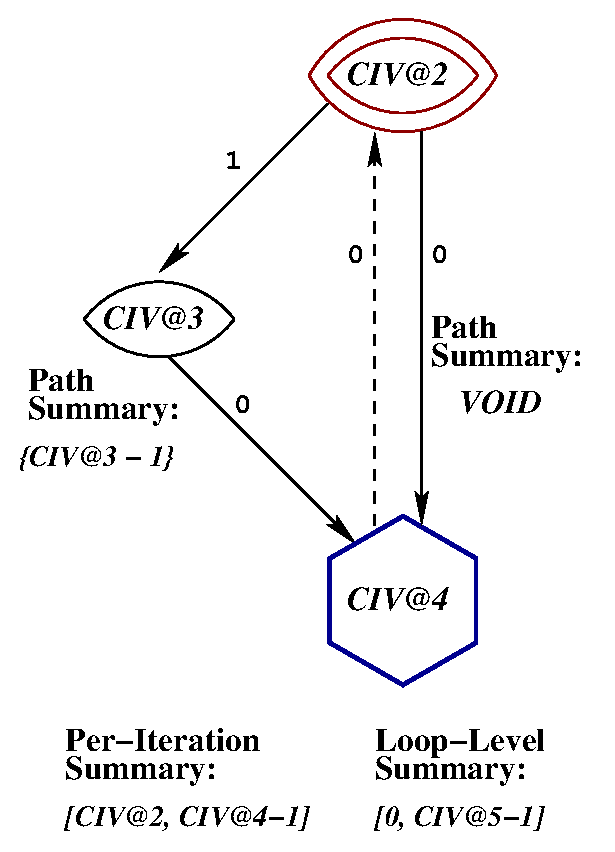
\includegraphics[width=.23\textwidth]{Figures/VEG_ACTFOR}
			} 
	} & { \hspace{-2ex}
			\subfigure[Loop {\tt CORREC\_do401}.]{ 
          			\label{fig:VegCORREC} 
          			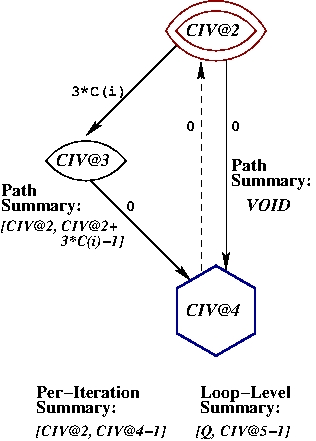
\includegraphics[width=.23\textwidth]{Figures/VEG_CORREC} 
			} 
	}
\end{tabular}
\caption{Summarizing CIV-based accesses at Gated-SSA Path, Iteration and Loop Levels.}
\vspace{-1ex}
\label{fig:AnonymousFig2} %
\end{figure}

\vspace{1ex}

{\bf 2. Projecting Summaries on VEG.}
The next stage is to project each gated-interval pair ${\tt g}\#L$ 
that contains {\sc civ} variables on its corresponding {\sc veg}\footnote{  
In principle, we may have ``regular'' gated-interval pairs, and also 
different pairs may correspond to {\sc civ}s from different {\sc veg}s. 
These are treated independently and the result is the union of partial results.
Analysis fails if one pair exhibits two {\sc civ}s belonging
to different {\sc veg}s.}. 
This corresponds to identifying the {\sc civ} node
that most-accurately describes the program point {\tt PP$_L$} 
where interval $L$ was summarized. 
One can observe that the naive choice of associating $L$ with the {\sc civ}
node that is used in $L$ is inaccurate: For example the gated-interval pair
corresponding to $\lceil WF_i \rceil$ in Figure~\ref{fig:codeActforCorrec}(b) 
is $[{\tt civ@2+1, civ@2+3*C(i)}]$, but node {\tt civ@3} 
is certainly a better choice than {\tt civ@2}, because associating
it with {\tt civ@2} would imply that the $WF_i$ summary also belongs 
to the path on which {\tt IA(j).NE.0} does not hold. 


Instead, we compute both the immediate {\sc civ}-node dominator and 
post-dominator of {\tt PP$_L$}, denoted by {\tt CIV}$_{d}$ and 
{\tt CIV}$_{pd}$, respectively, and chose {\tt CIV}$_{pd}$
as the projection node if {\tt CIV}$_{d}$ dominates {\tt CIV}$_{pd}$, 
and {\tt CIV}$_{d}$ otherwise. This guarantees that the {\sc civ} projection
is the ``closest'' node that belongs to any path passing through {\tt PP$_L$}
(the reverse does not hold).

The $\lceil WF_i\rceil$ overestimates of {\tt X} for the two 
examples of Figure~\ref{fig:codeActforCorrec}, namely
{\tt \{civ@3-1\}} and {\tt [civ@2,civ@2+3*C(i)-1]},
are both projected to node {\tt civ@3}. The annotated {\sc veg}s 
are shown in Figures~\ref{fig:VegACTFOR}~and~\ref{fig:VegCORREC}, respectively.
%
%With our examples in Figures~\ref{fig:codeActforCorrec}(a)~and~(b),
%intervals $\{{\tt civ@3-1}\}$ and $[{\tt civ@2},{\tt civ@2+3*C(i)-1}]$ 
%corresponding to $WF_i$'s  under and overestimate of array {\tt X} 
%are projected in both examples to node {\tt civ@3}.
%The annotated {\sc veg}s are depicted in 
%Figures~\ref{fig:VegACTFOR}~and~\ref{fig:VegCORREC}, respectively.

For underestimate computation it is {\em not enough} to associate an interval $L$ 
to a {\sc civ} node in the manner presented before, because it is not guaranteed
that any path that passes through the {\sc civ} node would also pass through {\tt PP$_L$}.
For example $L$ may summarize accesses of an inner-{\tt IF} branch 
(scope) that does not update the {\sc civ} variable. It follows that the {\tt IF} 
is not represented in the control-flow of the {\sc veg}, and it is incorrect
to consider $L$ part of the underestimate since the {\tt IF} branch might not be 
taken at runtime.

At this point we use the gate $g$ associated with $L$, which subsumes the
inner-{\tt IF} condition: In the computation
of an underestimate, a gated-interval $g\#L$ is considered part of a 
{\sc veg} path {\em iff the (total) condition of the {\sc veg} path}, i.e., 
the conjunction of all the $\gamma$-node gates on that path, {\em implies $g$}, 
i.e., the existence condition of $L$.  This guarantees that the summary belongs
to any control-flow path that includes the considered {\sc veg} path\footnote{
Establishing this invariant strictly from the control-flow graph is more
conservative, e.g., in our case the gates are translated/simplified across call sites,
hence more accurate.
%because the gates are aggressively simplified, e.g., across call sites, hence more accurate. 
}.
With our code, $g={\tt IA(j).NE.0}$ is identical to the gate of the path 
${\tt civ@2}\rightarrow{\tt civ@3}\rightarrow{\tt civ@4}$,
hence interval {\tt \{civ@3-1\}} safely belongs to this path.


\enlargethispage{\baselineskip}

\vspace{1ex}

{\bf 3. VEG-Path Summarization.} 
%
To compute the result on {\em one} path, all intervals are rewritten in terms of only the
{\sc civ}$_\mu$ node, by using the symbolic formulas of the path's evolution.
Then, all intervals belonging to the {\sc veg} path are united (unioned). 
If this succeeds, i.e., the result is one interval, then the resulting-interval upper 
bound is written in terms of the back node, {\sc civ}$_b$. If the result is free of
loop-variant symbols (other than {\sc civ}$_\mu$ and  {\sc civ}$_b$), such as {\tt 3*C(i)},
then the path-level analysis succeeds, otherwise it fails.

For example, the path ${\tt civ@2}\rightarrow{\tt civ@3}\rightarrow{\tt civ@4}$ 
of the {\sc veg} in Figure~\ref{fig:VegCORREC}, exhibits loop-variant evolution 
{\tt 3*C(i)}, and results in path interval {\tt [civ@2,civ@2+3*C(i)-1]}. 
%
However, rewriting the upper bound in terms of the back %$\mu$ and 
{\sc civ} node, results in $[{\tt civ@2},{\tt civ@4-1}]$,
i.e., we have performed substitution {\tt civ@2$\leftarrow$civ@4-3*C(i)}
derived from that path's evolution.
%since on that path ${\tt civ@4}={\tt civ@2+3*C(i)}$. 
It follows that aggregation succeeds.
%
Similarly, for the same path of the {\sc veg} in  Figure~\ref{fig:VegACTFOR}, the
path result is $\{{\tt civ@2}\}$, which is rewritten as
 $[{\tt civ@2}, {\tt civ@4-1}]$, since on that path 
${\tt civ@3}={\tt civ@2+1}$
and ${\tt civ@3}={\tt civ@4}$.

The other paths, for both {\sc veg}s, exhibit empty summaries and $0$ evolution,
i.e., {\tt civ@2=civ@4}. 
It follows that {\tt [civ@2, civ@4-1]~$\equiv \ \emptyset$} correctly 
describes them as well, i.e., an interval in which the upper bound is smaller 
than the lower bound is empty.
  As such, all paths share the same per-iteration result, in which the only 
non-constant terms are the $\mu$ and back {\sc civ} nodes, 
and analysis succeeds.


\vspace{1ex}

{\bf 4. Merge Across All Paths.} 
%
The last stage of the analysis is to compute the merge-over-all-paths result (interval).
%in a way consistent with the definitions of under and overestimate, respectively.
In our implementation the merge succeeds only when all path results are 
identical, which holds on both examples, e.g., $\lceil WF_i \rceil = {\tt [civ@2,civ@4-1]}$.
In the general case, one can compute the intersection/union over all paths as the  
under/overestimate result, respectively.
%Without loss of generality 
For simplicity, in the following, we assume that {\sc civ} values are monotonically 
increasing, and that the result's upper bound increases with the iteration number,
i.e., positive stride. 


We compute the total-union (loop) result as if we aggregate an affine access
across a loop whose lower and upper bounds are equal to the value of the 
{\sc civ} at the loop entry and exit, respectively.  
%
In our case this corresponds to replacing {\tt civ@2} and {\tt civ@4} 
with the {\sc civ} values at the loop entry and exit, in our case 
{\tt civ@1} and {\tt civ@5}, respectively. 
For both cases this yields result
{\tt [civ@1, civ@5-1]}.   If the sign of the {\sc civ} factor in
the affine-{\sc civ} expression is positive, then {\sc civ}'s
monotonicity ensures that the overestimate is correct. 

For the underestimate, correctness requires checking that the
per-iteration result $A_i$ is contiguous (or overlapping) 
between any two consecutive iterations. If $A_i=${\tt[lb$_i$,ub$_i$]$^s$},
this corresponds to checking that {\tt ub$_{i-1}$+s $=$ lb$_i$},
i.e., the upper bound of iteration {\tt i-1} plus the stride equals ($\leq$) 
the lower bound of iteration {\tt i}.
%
The check uses the invariant that the {\sc civ} value  
at the end of an iteration, i.e., the back node, equals 
the {\sc civ} value at the entry of the next iteration,
i.e., the $\mu$ node.
%
For $\lfloor WF_i \rfloor=${\tt [{\tt civ@2},{\tt civ@4}-1]$^1$},
this corresponds to replacing {\tt civ@4} with {\tt civ@2} in the upper bound 
and checking {\tt civ@2-1+1$=$civ@2}, which verifies statically. 

Note that in the case of Figure~\ref{fig:VegACTFOR},
the per-iteration result is a point, hence the stride is not set yet, and in
this case the stride is set to the value that verifies the invariant,
i.e., {\tt lb$_i$-ub$_{i-1}$}.
For example, if in Figure~\ref{fig:codeActforCorrec}(a) we would have 
{\tt civ@3=civ@2+2} instead of {\tt +1}, then the totally-aggregated
result would have stride {\tt 2}, i.e., {\tt [civ@1,civ@5-1]$^2$}.

Similarly, to compute the partial-loop-aggregation result, i.e., $\cup_{k=1}^{i-1}$,
we replace the {\sc civ} $\mu$ with the {\sc civ} node at the entry of the loop,
and the back node with the {\sc civ} $\mu$ node of iteration $i$, 
which results in interval {\tt[civ@1,civ@2-1]}.

Finally, if the over and underestimate results are identical then the result is
exact and the per-iteration or the partial/total aggregated result can be used
instead of $U_i$ or $\cup_{k=1}^{i-1} U_i$ or $\cup_{i=1}^n U_i$.  This is the
case with loop {\tt do j} in Figure~\ref{fig:codeActforCorrec}(a).  
%
The computed summaries allow now to prove the flow and output independence of the 
two loop examples, as we have already seen in Section~\ref{Intro:RelAppLim}.

\enlargethispage{\baselineskip}

\subsection{Enhancements to the Basic Technique}
\label{subsec:Track}


This section presents several refinements of the basic analysis,
that allow to parallelize several difficult loops, such as {\tt EXTEND\_do400} 
of {\tt track} benchmark. Since even the simplified code
is too complex for paper presentation, Figure~\ref{fig:VegEXTEND} presents the 
{\sc veg} of inner loop {\tt EXTEND\_do500}, which sheds significantly more 
insights than the code would do.


\begin{figure}[t]
    \begin{tabular}{ll} \hspace{-5ex} % @{\hspace{0.15\textwidth}}
	\multirow{2}{*}[29ex]
	{   
   		\subfigure[$\mbox{~~~~~~~~~~~~~~~~}$]{
          	\label{fig:USR_ROio_EXTEND_do500} 
			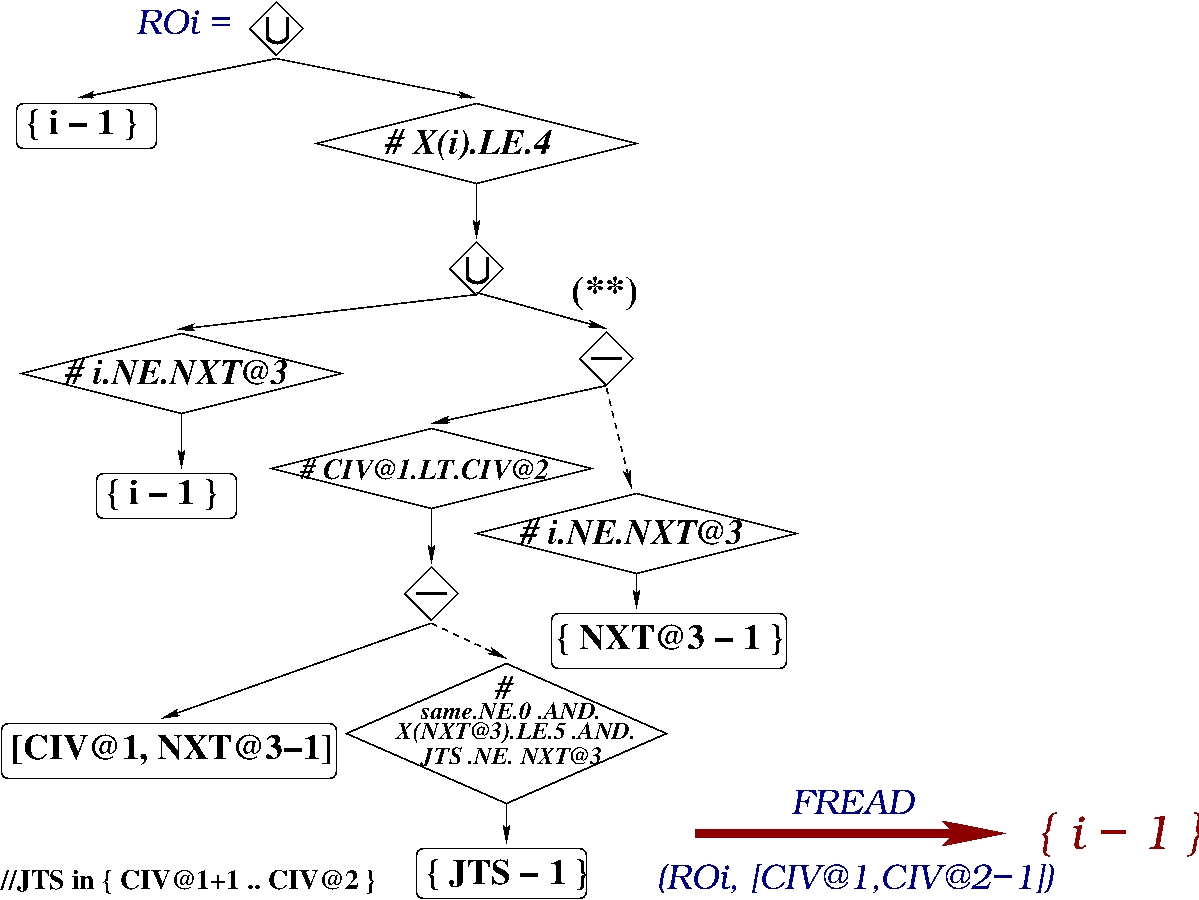
\includegraphics[width=.44\textwidth]{Figures/ROio_USR_EXTEND_do500}
	  	}
	} & {  \hspace{-31ex}
		\subfigure[$\mbox{~}$]{
          	\label{fig:VegEXTEND} 
			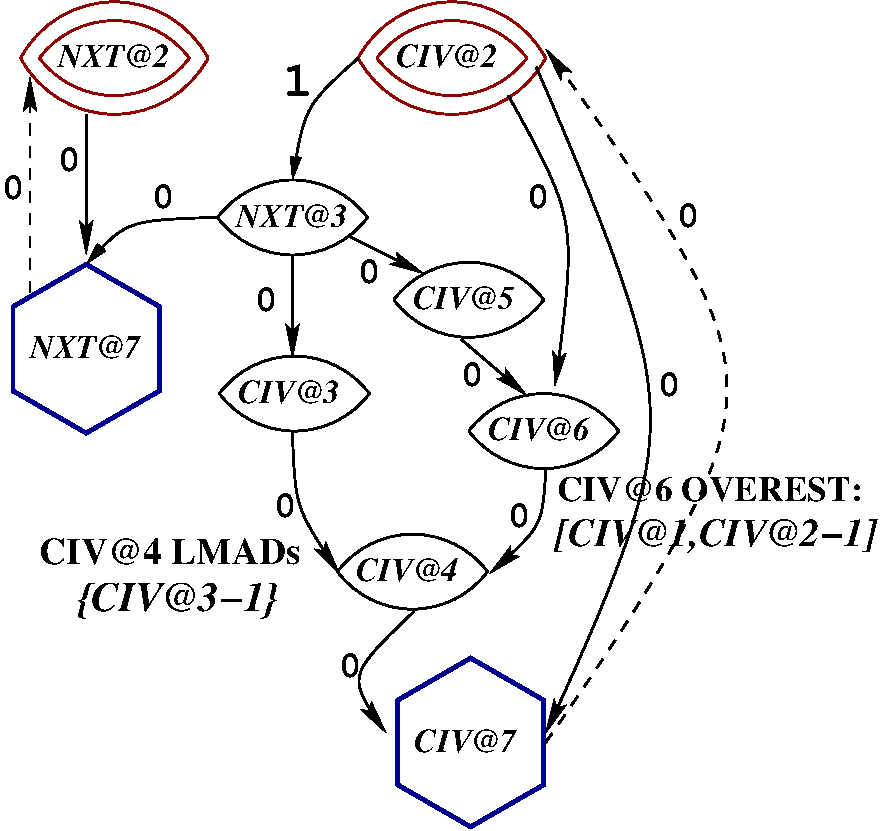
\includegraphics[width=.26\textwidth]{Figures/VEG_EXTEND}
	  	}
	}
    \end{tabular} \vspace{15ex} 
\vspace{-2ex}
\hrule
\caption{(a) {\sc ro}$_i$ {\sc usr} \& (b) {\tt civ}'s {\sc veg} for {\tt EXTEND\_do500}.} 
% Iteration-level 
%\caption{ {\sc wf}, {\sc ro}, {rw} abstract-set summarization across consecutive regions and loops.}
\label{fig:Track} %
\end{figure}
  
\vspace{1ex}

{\bf 1. Foreign Variables Allowed in VEG.}
%
One can observe in Figure~\ref{fig:VegEXTEND} that variable {\tt nxt@3} semantically 
contributes to the flow of {\tt civ} values, albeit it is a differently-named variable.
It follows that we allow {\tt nxt@3} to belong to the {\sc veg} rooted in the $\mu$ 
node {\tt civ@2}, especially since that {\sc veg} complies with the definition of a
{\sc civ} variable, which was given at the end of Section~\ref{subsec:Background}.
%
The analysis treats {\tt nxt@3} as any other member of the {\tt civ} family of 
variables, with {\em one notable exception}:  It is incorrect to allow summaries 
to be projected on foreign nodes such as {\tt nxt@3} because {\tt nxt@3}
is not accounted in the $\gamma$ nodes of {\tt civ}s, and, as such, does not
encapsulates the correct control flow.

\vspace{1ex}

{\bf 2. Filtering The Read Set}. The {\sc ro} ({\sc usr}) summary corresponding 
to iteration {\tt i} of loop {\tt EXTEND\_do500} is shown in 
Figure~\ref{fig:USR_ROio_EXTEND_do500}, where $\cup$, $-$ and $\#$ internal nodes 
correspond to set union, subtraction and gates, respectively.   
One can observe that {\sc ro}$_{i}$ is already nontrivial, e.g.,
contains both regular and {\sc civ}-based intervals (as leaves), and summarizing the 
{\sc ro} set at loop level by the rules in Figure~\ref{fig:LoopAggreg} would 
generate a complex, less-than-optimal set expression, e.g., for both proving 
independence and inferring accurate bounds for copy-in privatization.
%
We use instead a filtering technique based on the observation that
the contribution of {\sc ro}$_i$ to the loop-aggregated
{\sc ro} set cannot possibly belong to $\cup_{k=1}^{i-1}${\sc wf}$_k$.
%(because it would necessarily belong to the {\sc wf}-aggregated set). 
The same property holds for the read-write set.

\begin{figure}[t]
\begin{scriptsize}
USR {\bf FREAD}($R$ : USR, $WF^p$ : LMAD) \vspace{1ex} \newline
$\mbox{ }\mbox{ }$// {\bf {\em Output:}} $R$ filtered-out of $WF^p$ terms. \vspace{1ex} \newline
$\mbox{ }\mbox{ }$Case $R$ of: \vspace{1ex} \newline
$\mbox{ }\mbox{ }\mbox{ }\mbox{ }$ LMAD $L$: %\vspace{1ex} \newline
%$\mbox{ }\mbox{ }\mbox{ }\mbox{ }\mbox{ }\mbox{ }$ 
{\bf IF} $\mathcal{F}(L - WF^p)$ {\bf THEN} $\emptyset$ {\bf ELSE} $L$ \vspace{1ex} \newline
$\mbox{ }\mbox{ }\mbox{ }\mbox{ }$ $g\#A$: $g\#${\bf FREAD}($A$,$WF^p$)  \vspace{1ex} \newline   
$\mbox{ }\mbox{ }\mbox{ }\mbox{ }$ $A \cup B$: {\bf FREAD}($A$,$WF^p$) $\cup$ {\bf FREAD}($B$,$WF^p$) \vspace{1ex} \newline
$\mbox{ }\mbox{ }\mbox{ }\mbox{ }$ $A \cap B$: {\bf FREAD}($A$,$WF^p$) $\cap$ {\bf FREAD}($B$,$WF^p$) \vspace{1ex} \newline
$\mbox{ }\mbox{ }\mbox{ }\mbox{ }$ $A - B$: {\bf FREAD}($A$,$\lfloor B \rfloor \cup WF^p$)   \vspace{1ex} \newline
$\mbox{ }\mbox{ }\mbox{ }\mbox{ }$ LOOP OR CALLSITE :   \vspace{1ex} \newline   
$\mbox{ }\mbox{ }\mbox{ }$ 
$\mbox{ }\mbox{ }\mbox{ }$ 
          {\bf IF}($\mathcal{F}$($\lceil R \rceil - WF^p$) THEN $\emptyset$ ELSE $R$ \vspace{1ex} \newline
\end{scriptsize}
\hrule
\caption{ Read-Set Filtering Algorithm.}
\label{fig:ReadFilt} %
\end{figure}


Figure~\ref{fig:ReadFilt} shows the recursively-defined operator {\tt FREAD} that
filters out from the {\sc ro}$_i$ ({\sc rw}$_i$) set, the terms that are included 
into an interval underestimate of $\lfloor\cup_{k=1}^{i-1}${\sc wf}$_k\rfloor$, 
denoted $WF^p$.
%, from the {\sc ro}$_i$ and {\sc rw}$_i$ sets. 
The result summary replaces {\sc ro}$_i$ in Figure~\ref{fig:LoopAggreg}'s equations.

If the current node of {\sc ro}$_i$ is an interval ({\sc lmad}) $L$ then we extract a 
sufficient predicate for $L - WF^p = \emptyset$ by using the {\sc usr}-to-predicate
translation $\mathcal{F}$ mentioned in Section~\ref{subsec:Background}.   
If the predicate statically evaluates to {\tt true} then it is safe to 
filter $L$ out, otherwise $L$ (or $L-WF^p$) is kept.  
%
Similarly, if the current node, named $R$, is a loop or callsite node, 
then we check using $\mathcal{F}$ whether an interval overestimate of 
$R$ is included in $WF^p$; if so then $R$ is filtered out, otherwise 
it is kept.  
%
If $R$ is a gate or union or intersection node,
then each term is filtered and the results are composed back. 
%
If $R$ is a subtraction node $A-B$ then $A$ is filtered with the union 
of $WF^p$ and an interval underestimate of $B$. 

Filtering the $RO_{i}$ set depicted in Figure~\ref{fig:USR_ROio_EXTEND_do500}
with the computed $\lfloor \cup_{k=1}^{i-1}WF_k\rfloor={\tt [civ@1,civ@2-1]}$
results in the simple $RO'_{i} = {\tt\{i-1\}}$, where the problematic 
subtraction node, denoted by {\tt (**)} in Figure, has been simplified\footnote{
The algorithm has used the {\sc veg}-derived properties (i) ${\tt civ@1} < {\tt jts} \leq {\tt civ@2}$ 
and (ii) ${\tt M} \leq {\tt civ@1}$, where {\tt civ@1} is the {\sc civ} value 
just before entering the loop, and {\tt M} is the loop upper bound. Since 
{\tt civ}-values are monotonically increasing, it also follows: 
{\tt i $\leq$ M $\leq$ civ@1 $\leq$ civ@2 $<$ nxt@3.}
}
to $\emptyset$.%Similarly $RW'_{i} = \emptyset$.


\vspace{1ex}

{\bf 3. Output-Dependence Pattern.} 
%
{\tt EXTEND\_do400} exhibits per-iteration and partial-recurrence {\sc wf} 
sets of shape:\\
\noindent$\lceil WF_i\rceil = $ {\tt[civ@1,civ@8~~]},
$\lceil\cup_{k=1}^{i-1}WF_{k} \rceil = $ {\tt[civ,civ@1~~]},\\
\noindent$\lfloor WF_i\rfloor = $ {\tt[civ@1,civ@8-1]},
$\lfloor\cup_{k=1}^{i-1}WF_k \rfloor = $ {\tt[civ,civ@1-1]},\\
where {\tt civ@1} and {\tt civ@8} are the $\mu$ and back nodes of
the {\sc veg} associated to loop {\tt EXTEND\_do400} and variable {\tt civ}.
%
One can observe that output-dependencies may exist, since
the output-independence equation of Figure~\ref{fig:IndEq} is not satisfied:
$\lceil WF_{i}\rceil \cap \lceil \cup_{k=1}^{i-1}WF_{k} \rceil \equiv {\tt\{civ@1\}}\ne\emptyset$.
(This behavior is caused by a {\tt 0}-evolution path on which the array is updated,
and which causes cross-iteration output dependencies.)

Still, dependencies exhibit a well-structured pattern that our 
implementation exploits. The key observations are: 
\begin{itemize}
    \item Indices belonging to $\lfloor{}WF_{j}\rfloor$ underestimate  
            do not result in cross dependencies:
        $\lfloor WF_{i}\rfloor\mbox{~}\cap\mbox{~}\cup_{k=1}^{i-1}\lfloor WF_{k}\rfloor~=~\emptyset$.

    \item All remaining indices, 
        $\lceil WF_{i}\rceil - \lfloor WF_{i}\rfloor = {\tt\{civ@8\}}$,
        are overwritten by the next {\sc civ}-increasing iteration:
        {\tt{}civ@8>civ@1} $\Rightarrow$
        {\tt\{civ@1\}} $\subseteq\lfloor WF_{i}\rfloor${\tt=[civ@1,civ@8-1]},
        %
        where {\tt\{civ@8\}} of the previous iteration was written as 
        {\tt\{civ@1\}} of the next {\sc civ}-increasing iteration.

    \item Last iteration increases the {\sc civ} value; this 
        holds for {\tt EXTEND\_do400} because {\sc civ} is 
        updated in an inner loop.
\end{itemize}

%verified at runtime via predicates.
If all properties hold, then the output-dependency pattern is resolved 
by privatizing the array (updates) and by copying out, at iteration's
end, the indices belonging to the $\lfloor WF_i\rfloor$ 
underestimate, i.e., {\tt[civ@1,civ@8-1]}.
The last iteration writes directly to global storage, and because
it increases {\sc civ}, it is guaranteed to overwrite the uncommitted 
part of previous (non-increasing) iterations.
%
The last property is verified at runtime, during the {\sc civ}-value
(pre)computation, while the first two are derived statically 
for the current loop, but in general, they may also use runtime verification.

\vspace{1ex}
{\bf 4. Privatizable Stack.} Our analysis also extends (with
some modifications) to a stack-like access pattern in which
the {\sc civ} values are only piecewise monotonic.
This is discusses in Appendix~\ref{sec:Stack} in the
context of loop {\tt ACCEL\_do10} from {\tt tree} benchmark
that exhibits a privatizable stack. 


\subsection{CIV$_\mu$ Computation \& Implementation }
\label{subsect:CivImplem}

The independence results discussed in previous sections have referred 
so far to disambiguating array accesses that exhibit {\sc civ} 
subscripts, but not to the computation of the {\sc civ} values.
%
When the {\sc civ} variable is not privatisable in the context of the 
target loop, e.g., the loop in Figure~\ref{fig:codeActforCorrec}(b), 
the {\sc civ} is the source of cross-iteration flow dependencies: %in essence 
it is always updated in reduction-like statements, e.g., {\tt civ=civ+3*C(i)},
but it is read in arbitrary statements, e.g., in a subscript.


While not always necessary~\cite{PaduaStackArr}, we  (pre)compute in %always 
parallel, prior to loop execution, the {\sc civ}$_\mu$ values at the beginning 
of each (chunk of) iteration(s).
Reasons are threefold: {\em First}, in most cases %it is cleaner to do so, and 
the runtime overhead is small. {\em Second}, the {\sc civ} values may dictate
whether the loop is independent or not: For example,  the flow-independence
predicate of the loop in Figure~\ref{fig:codeActforCorrec}(b), 
${\tt N} \le {\tt Q}~\vee~{\tt civ@5} < {\tt M}$,
depends on {\tt civ@5}, while resolving statically the output 
dependencies of {\tt EXTEND\_do400}, depends, as
per Section~\ref{subsec:Track}, on establishing whether the last
iteration has increased the {\sc civ} value. 
%
{\em Third}, {\sc civ} values may flow in the computation
of data (rather than only subscripts), e.g., the recurrent
formula of the Sobol random number generator, used in
benchmark {\tt Pricing}  of Section~\ref{sec:EmpEval}.

{\sc civ}$_\mu$ values are (pre)computed by extracting the loop-slice
that contains the transitive closure of all statements 
that are necessary to compute the {\sc civ} variable
(we use the control-dependency graph). 
We privatize all arrays and scalars, including {\sc civ}, that are not 
read-only inside the slice, where each iteration copies-in the  indices 
of its $RO_i \cup RW_i$ set. Finally, an iteration-header statement is 
inserted to initialize {\sc civ} to the value just before the loop ({\tt Q}), 
and similarly, the end-of-iteration value minus {\tt Q} is saved into array 
{\tt CIVS}.  


\begin{figure}
\begin{colorcode}
//\mymath{slice for computing partial civ values}
DOALL i = M, N, 1      \$PRIVATIZED(civ,i)
  civ = Q
  IF ( C(i) .GT. 0 ) civ = civ + 3*C(i)
  CIVS(i-M+1) = civ - Q
ENDDOALL

//\mymath{SCAN(op {\tt{}+}, e, n, {\tt{}X}) \equiv} \{\mymath{e}, \mymath{e}+X(1),.., \mymath{e}+X(1)+..+X(n)\}
SCAN(op +, Q, N-M+1, CIVS)

//\mymath{civ values are plugged in the loop}
DOALL i = M, N, 1      \$PRIVATIZED(civ,i)
  civ = CIVS(i-M+1)
  ... \mymath{rest of the loop code}
ENDDOALL
\end{colorcode}
\vspace{-1ex}
\hrule
\vspace{-0.5ex}
\caption{ Parallel (Pre)Computation of {\sc civ}$_\mu$ Values.}
\label{fig:CivSlice} %
\end{figure}

For example, Figure~\ref{fig:CivSlice} shows the {\sc civ} slice of the loop
in Figure~\ref{fig:codeActforCorrec}(b), where scalars {\tt i} and {\tt civ}
were privatized. The slice computes the per-iteration {\sc civ} increments 
and records them in {\tt CIVS}. Then {\tt SCAN}
computes in parallel the prefix sum of the {\tt CIVS} values, 
hence the {\sc civ}$_\mu$ values at the beginning of each iteration. 
%
Requirements for correctness are {\em twofold}:  

{\em First}, all symbols that appear in the slice have been already proven 
to not introduce cross-iteration dependencies in the original loop; otherwise 
the computation of the slice might violate the semantics of the sequential execution. 

{\em Second}, {\sc civ} variables may appear in the slice only in reduction-like statements, 
such as {\tt civ=civ+1}.
If this holds than the final {\sc civ} value would correspond to an (additive) reduction, 
and hence, the intermediate {\sc civ}$_\mu$ values are safely computed via the parallel 
prefix sum of the values in {\tt CIVS}. 

If the latter does not hold, %than we are inside a vicious circle:
%the {\sc civ} computation depends on the {\sc civ} values 
%that we are about to compute. 
then we have a cycle between {\sc civ}-value computation and their use.   
We address such a case via a fixed-point implementation,
which (i) optimistically computes the {\sc civ} values as before, and then (ii) logically 
re-executes the slice on the computed-{\sc civ} values and checks (in parallel) 
whether the resulted value matches the input-value of the next iteration. 
%
If the check succeeds across all iterations, one can prove correctness by induction:
The first iteration is always correct. If the value at the end of the first iteration 
coincides with the input of the second, then the second iteration 
is correct, etc.%guaranteed to be correct, and so on.   

%We observe that the fix-pointed verification could be integrated in the 
%(parallel, optimistic) execution of the original loop: Rather than running the slice twice,
%we run the loop in a copy-in, copy-out policy, and if the verification fails then, 
%instead of copying-out the result arrays, the loop is re-executed sequentially.

Finally, {\sc civ}$_\mu$ input values are plugged in the 
parallel execution of the original loop: The arrays that were proven flow and output
independent are shared, i.e., not privatized.   For cases such as {\tt EXTEND\_do400},
that exhibit the special pattern of output dependencies, we adopt a strategy similar
to the one used for {\sc civ} computation: arrays such as {\tt X} are privatized,
their read-set {\sc ro}$_i$ $\cup$ {\sc rw}$_i$ is copied in, and the per-iteration {\sc wf} underestimate
is copied-out at the iteration's end.   Our technique is deeply integrated with the
underlying compiler framework: On the one hand, $\mathcal{F}$ uses the {\sc civ}-summarized
over and underestimates to derive sufficient-independence predicates.
%
On the other hand $\mathcal{F}$ is used in the summarization process, for example 
to simplify the {\sc ro}/{\sc rw} per-iteration sets, and thus to optimize the 
size of the data that needs to be copied in.  Similarly, Fourier-Motzkin-like
elimination reduces both loop indices and {\sc civ}s, i.e., when {\sc civ}'s 
bounds are derivable from its {\sc veg}. %in its corresponding {\sc veg}.



\section{Experimental Evaluation}
\label{sec:EmpEval}

\begin{table}[t] 
\centering
\scriptsize   
\begin{tabular}{|c|l|l|c|c|l|} \hline
\multicolumn{6}{|c|}{Properties of Benchmarks Exhibiting Important Loops That Use {\sc civ}s} \\ \hline
{\sc bench} & {\sc properties} & {\sc do loop}  & {\sc lsc}\%  & T$_{P/S}^L$(s) & {\sc type} \\ \hline
{\sc bdna}  &  T$_{P/S}$=.25/.65 s         & {\sc actfor\_500}  & 47.8 & .09/.31 & {\sc st-par}     \\ 
{\tt P=4}         &  {\sc sc}=87\%,{\sc ov}=0\%  & {\sc actfor\_240}  & 35.6 & .07/.23 & {\sc civ}$_{\tt{}AGG}$    \\ \hline 
             &  T$_{P/S}$=1.3/3.1 s         & {\sc gmttst\_120}  & 17.4 & .27/.54 & {\sc {\sc fi} {\sc o(1)}}   \\ 
{\sc nasa7}  &  {\sc sc}=98\%,{\sc ov}=0\%  & {\sc emit\_5}      & 13.6 & .17/.42 & {\sc civ}$_{\tt{}COMP}$   \\  % ,{\sc oi} {\sc o(n)}
{\tt P=4}        &                              &                      &                & & {\sc oi} {\sc o(n)}       \\
             &                              & {\sc btrtst\_120}  & 10.1 & .08/.31 & {\sc fi} {\sc o(1)}        \\ \hline
{\sc track}  &  T$_{P/S}$=6.6/16.8 s         & {\sc fptrak\_300}  & 52.8 & 3.6/8.9 & {\sc civ}$_{\tt{}COMP}$   \\ 
{\tt P=8}        &  {\sc sc}=97\%,{\sc ov}=45\%  & {\sc extend\_400}  & 43.9 & 2.3/7.4 & {\sc civ}$_{\tt{}COMP}$ \\ \hline 
{\sc tree}   &  T$_{P/S}$=12.8/59 s        & {\sc accel\_10}    & 91.2 & 7.6/54 & {\sc civ}$_{\tt{}AGG}$  \\            %58.6%53.5
{\tt P=8}        &  {\sc sc}=91\%,{\sc ov}=0\% &                    &      &          &                           \\ \hline 
{\sc price\_i} &  T$_{P/S}$=.29/2.0 s        & {\sc price\_i\_10} & 99   & .29/2.0  & {\sc civ}$_{\tt{}AGG}$ \\ 
{\tt P=8}          &  {\sc sc}=99\%,{\sc ov}=0\% &                    &      &          &                           \\ \hline 
{\sc price\_r} &  T$_{P/S}$=.17/.98 s          & {\sc price\_r\_10}& 99   & .17/.98  & {\sc civ}$_{\tt{}COMP}$ \\ 
{\tt P=8}          &  {\sc sc}=99\%,{\sc ov}=6.4\% &                  &      &          &                          \\ \hline 
\end{tabular}
\caption{ Characterization of Important CIV Loops.
%            Table's Layout Is Explained at the Start of Section~\ref{sec:EmpEval}. 
}
\label{tab:LoopBenchProps}
\end{table}


We evaluate our technique on a number of benchmarks containing loops that cover a significant
fraction of the total sequential runtime and that exhibit {\sc civ}-based accesses.
%
Table~\ref{tab:LoopBenchProps} characterizes several representative loops, named in 
the third column, and their corresponding benchmarks, named in the first column.
{\tt P=4} or {\tt 8} in the benchmark column shows the number of cores used for 
parallel execution. 
%
%The last column shows the number of cores used for parallel execution. 
Benchmarks {\tt bdna} and {\tt nasa7}
%, which belong to the {\sc perfect-club} and {\sc spec2000} suites,
were run on (only) four cores because they exhibit small data sets, i.e., low-granularity 
loops, that limit the profitability of parallelization. 
In addition, (i) loop {\tt GMTTST\_do120} 
%from {\tt nasa7} 
is parallel but has loop-count three, and (ii) loop {\tt RESTAR\_do15},
%from {\tt bdna}, 
which covers $9.3\%$ of the sequential runtime, uses {\sc io} operations,
and was run sequentially. The other benchmarks use eight cores.


The second column shows 
(i)   the parallel and sequential runtime, T$_{P/S}$, measured in seconds,
(ii)  the percentage, {\sc sc}, of the sequential runtime that has been parallelized, and 
(iii) the overhead of the associated runtime tests, if any, which is represented as percentage of
        the total-parallel runtime. With our benchmarks, the only runtime test that introduces
        non-negligible overhead is the (pre)computation of {\sc civ} values, 
        denoted {\sc civ}$_{\tt{}COMP}$, and presented in Section~\ref{subsect:CivImplem}.   

The fourth column shows the sequential coverage, {\sc lsc}, of each loop, and the
fifth column shows each loop's parallel and sequential runtime, T$_{P/S}^L$, in seconds.

The sixth column shows {\em how} the loop was classified parallel: {\sc fi} {\sc o(1)}
means that a predicate of runtime complexity {\sc o(1)} has validated loop's flow
independence at runtime. {\sc civ}$_{\tt{}AGG}$ indicates that {\sc civ}-based summarization 
was instrumental in proving independence statically, and {\sc civ}$_{\tt{}COMP}$ means that,
in addition to {\sc civ}$_{\tt{}AGG}$, the {\sc civ}$_\mu$ values were precomputed
at runtime, i.e., {\sc civ} was not privatizable.  {\sc st-par} indicates static
parallelization of a ``regular'' loop. 



%%% orig .37\textwidth  35ex
\begin{figure*}[t]
	\begin{tabular}{c c c} 
\multicolumn{2}{}{} 
	\multirow{2}{*}[32ex]
	{      		%\hspace{-6ex}	
                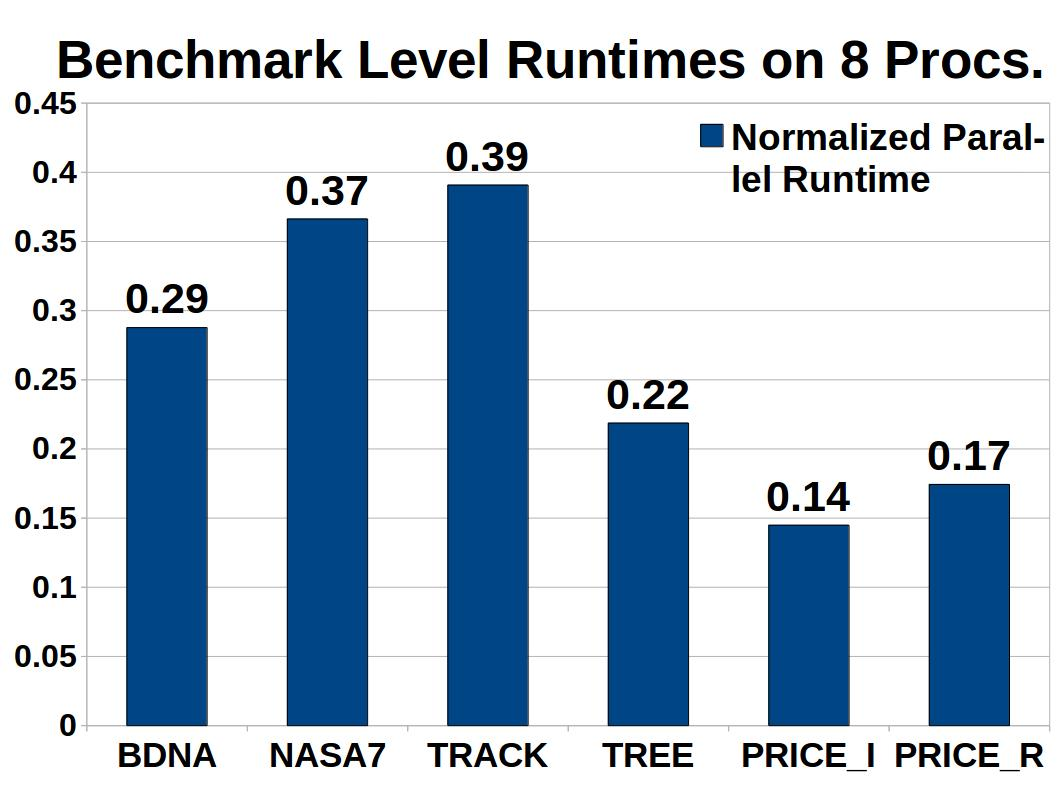
\includegraphics[width=.35\textwidth]{Figures/EmpRes/BenchParRes} \vspace{2ex}     
	} & { \hspace{-55ex}
                    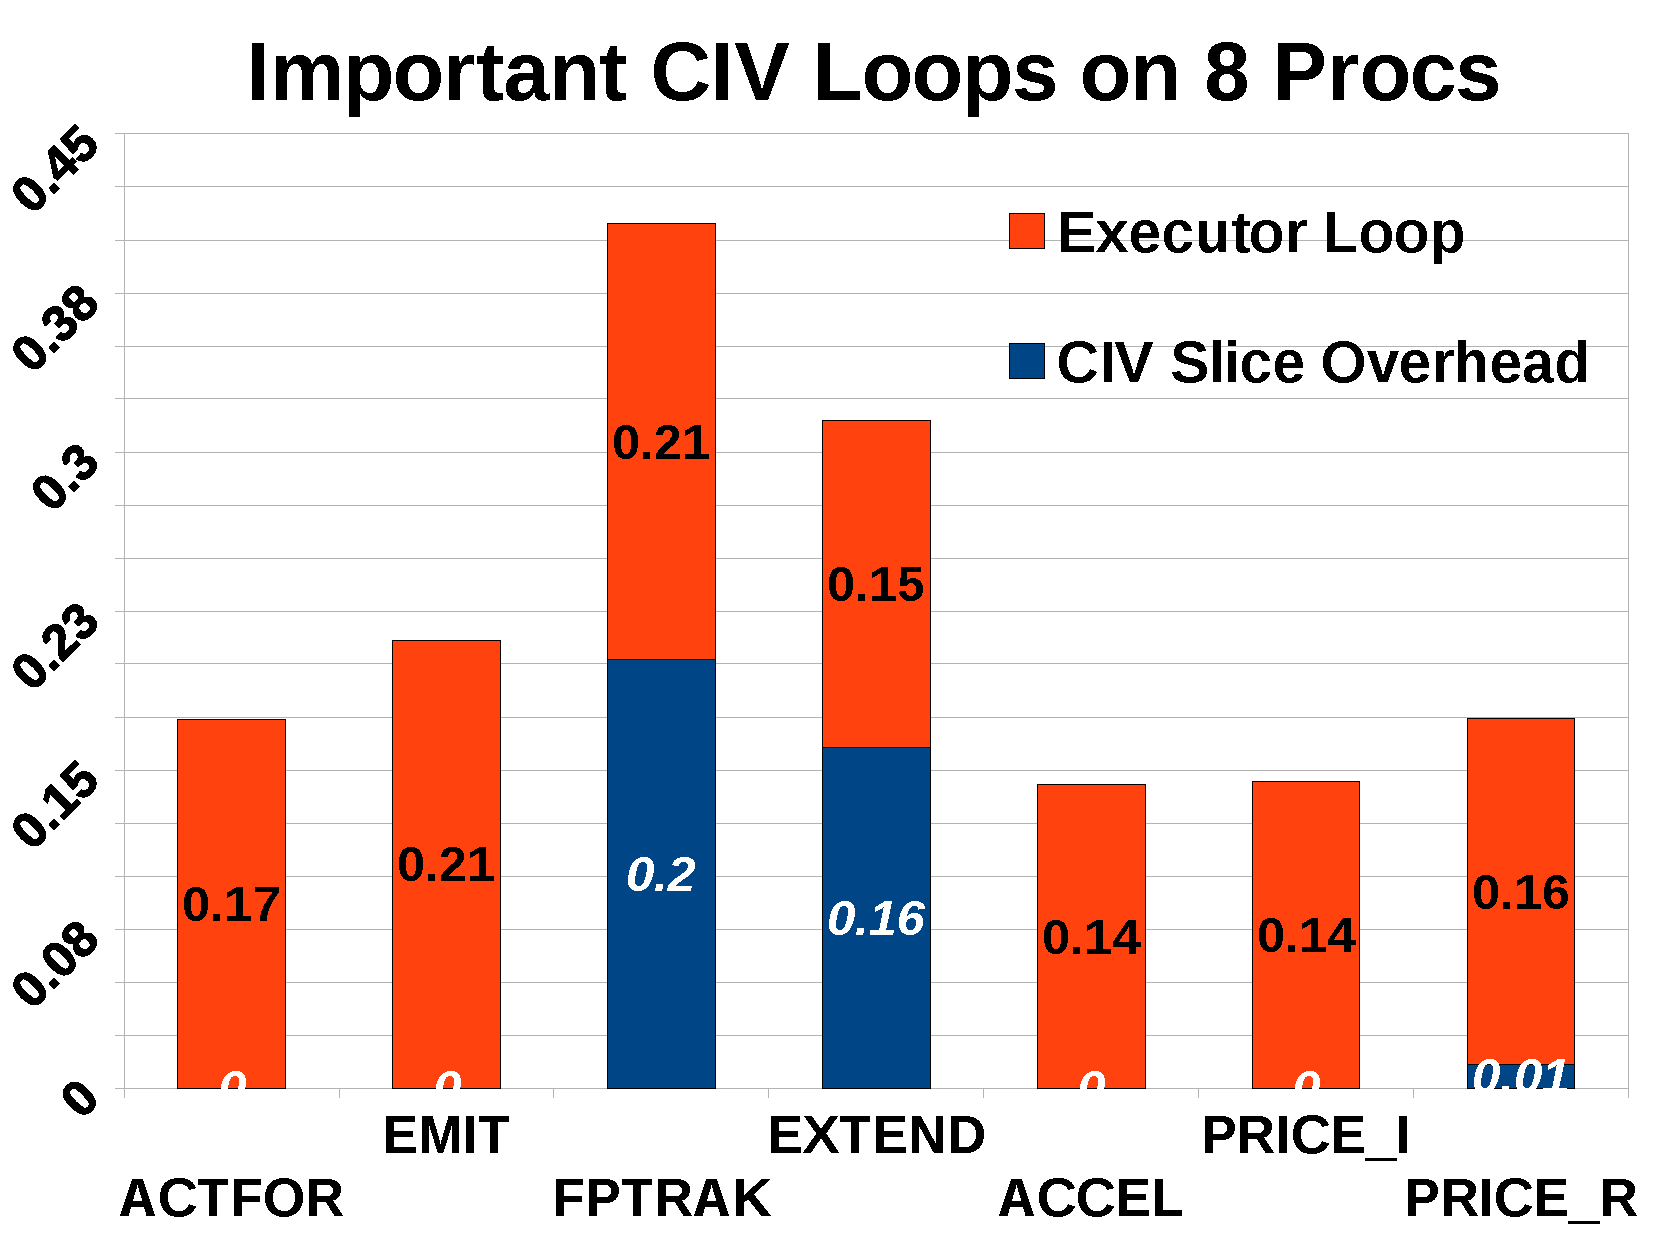
\includegraphics[width=.35\textwidth]{Figures/EmpRes/LoopParRes} \vspace{2ex}
	} \\ 
	\multirow{2}{*}[32ex]
	{           
                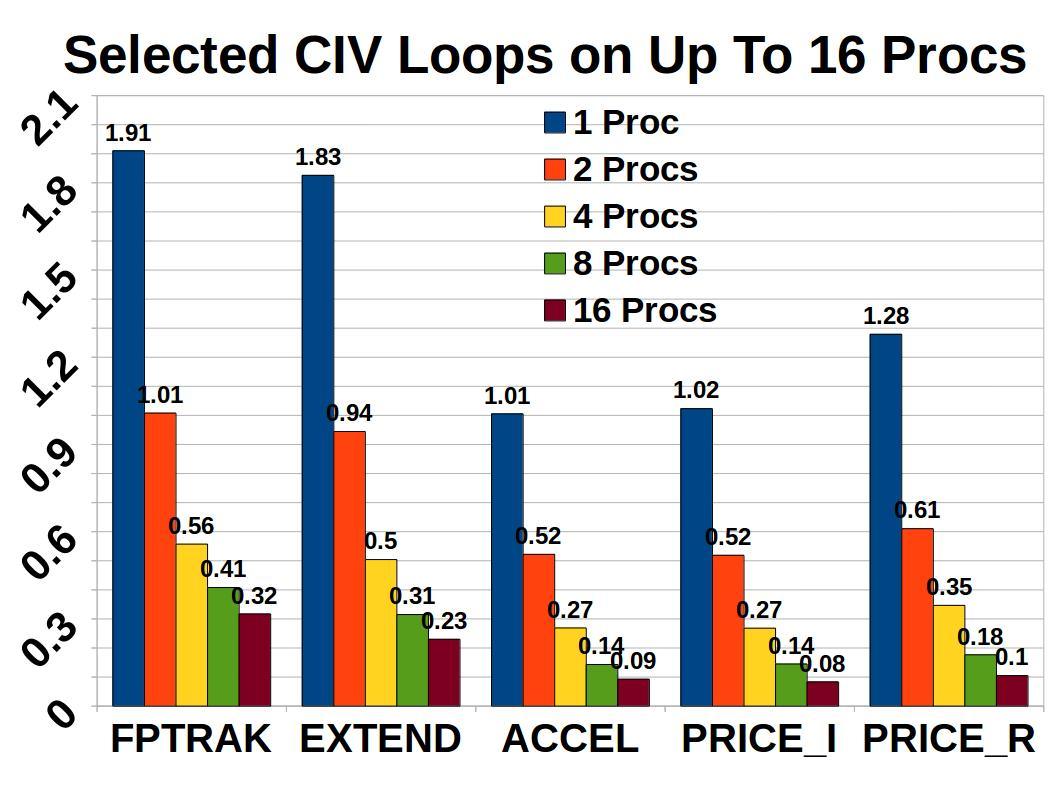
\includegraphics[width=.35\textwidth]{Figures/EmpRes/LoopScalRes}
	} & { \hspace{16ex}
                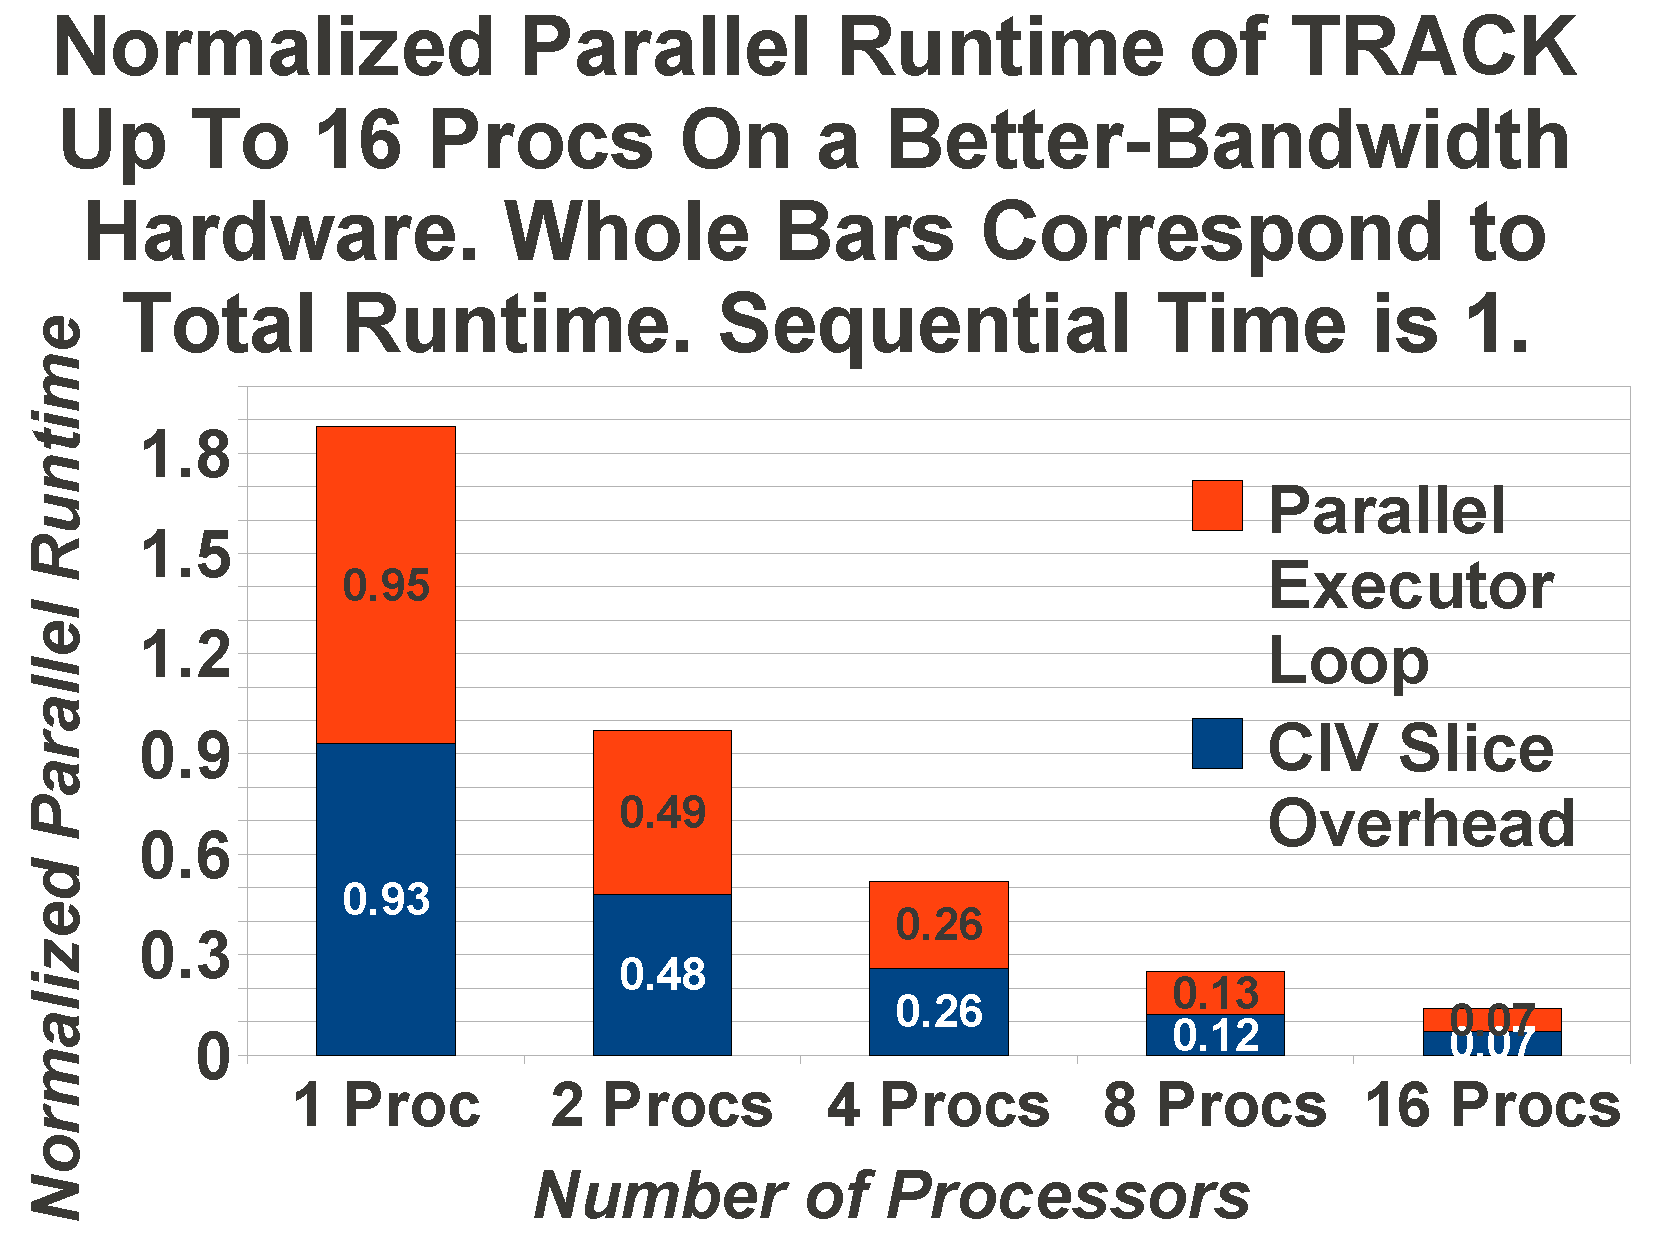
\includegraphics[width=.35\textwidth]{Figures/EmpRes/TrackScalNew}
	}
\end{tabular}
\hrule
\caption{ Benchmark and Loop-Level Normalized Runtime and Scalability Results. }
\label{fig:ParRuntime} %
\end{figure*}


\vspace{1ex}

{\bf Our Test Suite} consists of benchmarks {\tt bdna} and {\tt track} 
from {\sc perfect-club} suite, whose loops have been already discussed;
loop {\tt FPTRAK\_do300} from {\tt track} is similar to {\tt EXTEND\_do400},
%in Figure~\ref{fig:EXTEND}, 
and loop {\tt CORREC\_do401} is not shown because 
its sequential coverage is under $1\%$. 
%
Benchmark {\tt nasa7} is part of {\sc spec2000} suite, and its loop {\tt EMIT\_do5}
is similar to the one in Figure~\ref{fig:codeActforCorrec}(b).
%
Benchmark {\tt tree}~\cite{Treecode} is an implementation of the Barnes-Hut algorithm.
Its main loop, {\tt ACCEL\_do10}, exhibits the stack-access pattern of Figure~\ref{fig:Tree}(a),
and accounts for $91\%$ of the sequential runtime. The remaining $9\%$ corresponds to {\sc io}
operations and cannot be parallelized.
%
Finally,  {\tt price\_i/r} is a (simplified) kernel of a real-world application that
computes the price of a financial contract~\cite{LexiFiPricing}:   The difference
between the two versions is that (i) {\tt price\_i} uses an independent Sobol-random-number-generator
algorithm, i.e., computing the $i^{th}$ random number requires only the value of $i$,
and exhibits the {\sc civ} pattern of Figure~\ref{fig:codeActforCorrec}(a), 
while (ii) {\tt price\_r} uses a faster, recurrent formula that computes the 
$i^{th}$ random number based on the previous $(i-1)^{th}$ one. 
Parallelization of {\tt price\_r} consists of (pre)computing
in parallel these {\sc civ}$_\mu$ values, in the manner of 
Section~\ref{subsect:CivImplem}.  

%\begin{figure}[t]
%	\begin{tabular}{l l l} 
%\multicolumn{2}{}{} 
%	\multirow{2}{*}[24ex]
%	{      		\hspace{-6ex}	
%                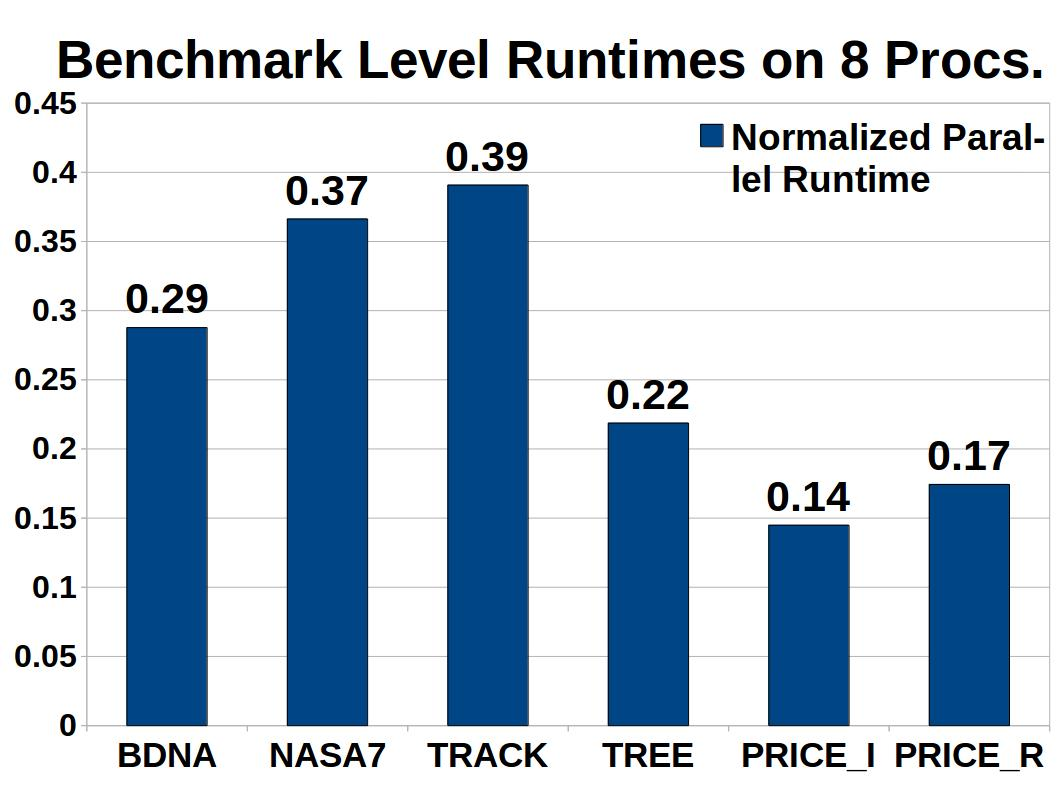
\includegraphics[width=.27\textwidth]{Figures/EmpRes/BenchParRes} \vspace{2ex}     
%	} & { \hspace{-39ex}
%                    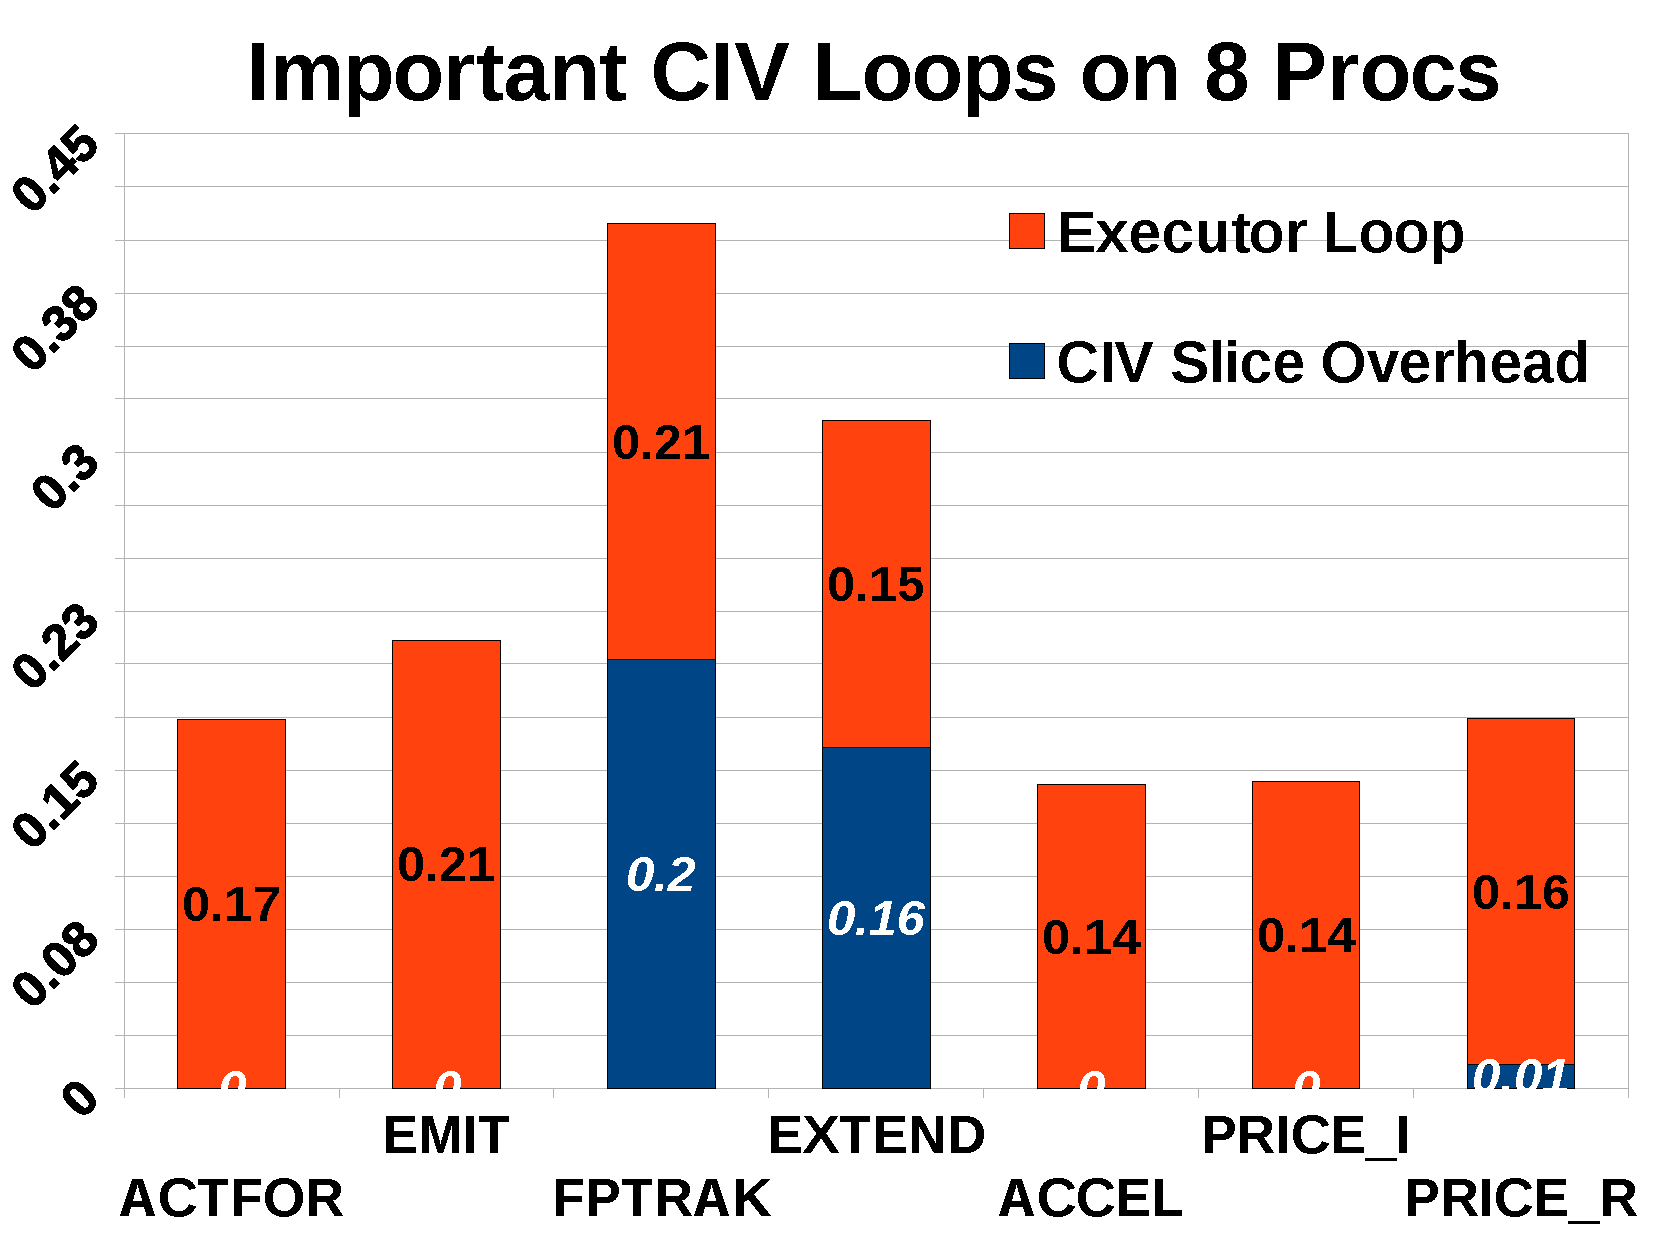
\includegraphics[width=.27\textwidth]{Figures/EmpRes/LoopParRes} \vspace{2ex}
%	} \\ 
%	\multirow{2}{*}[24ex]
%	{           \hspace{-7ex} 
%                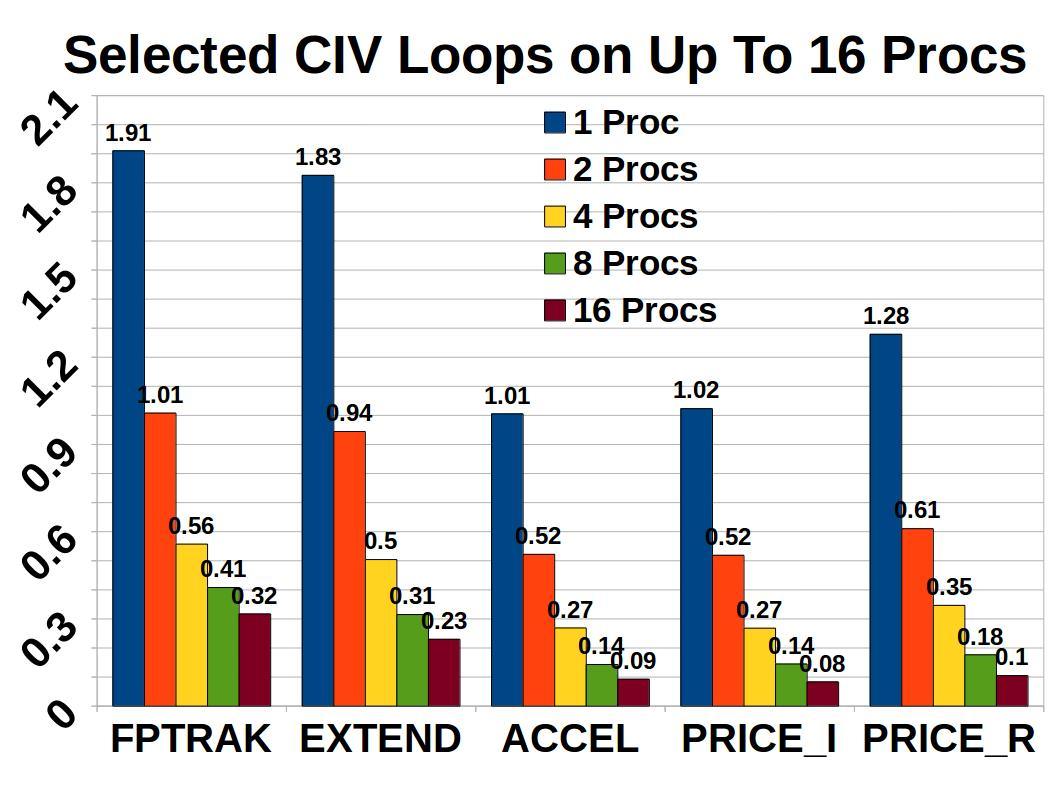
\includegraphics[width=.27\textwidth]{Figures/EmpRes/LoopScalRes}
%	} & {       \hspace{-5ex} 
%                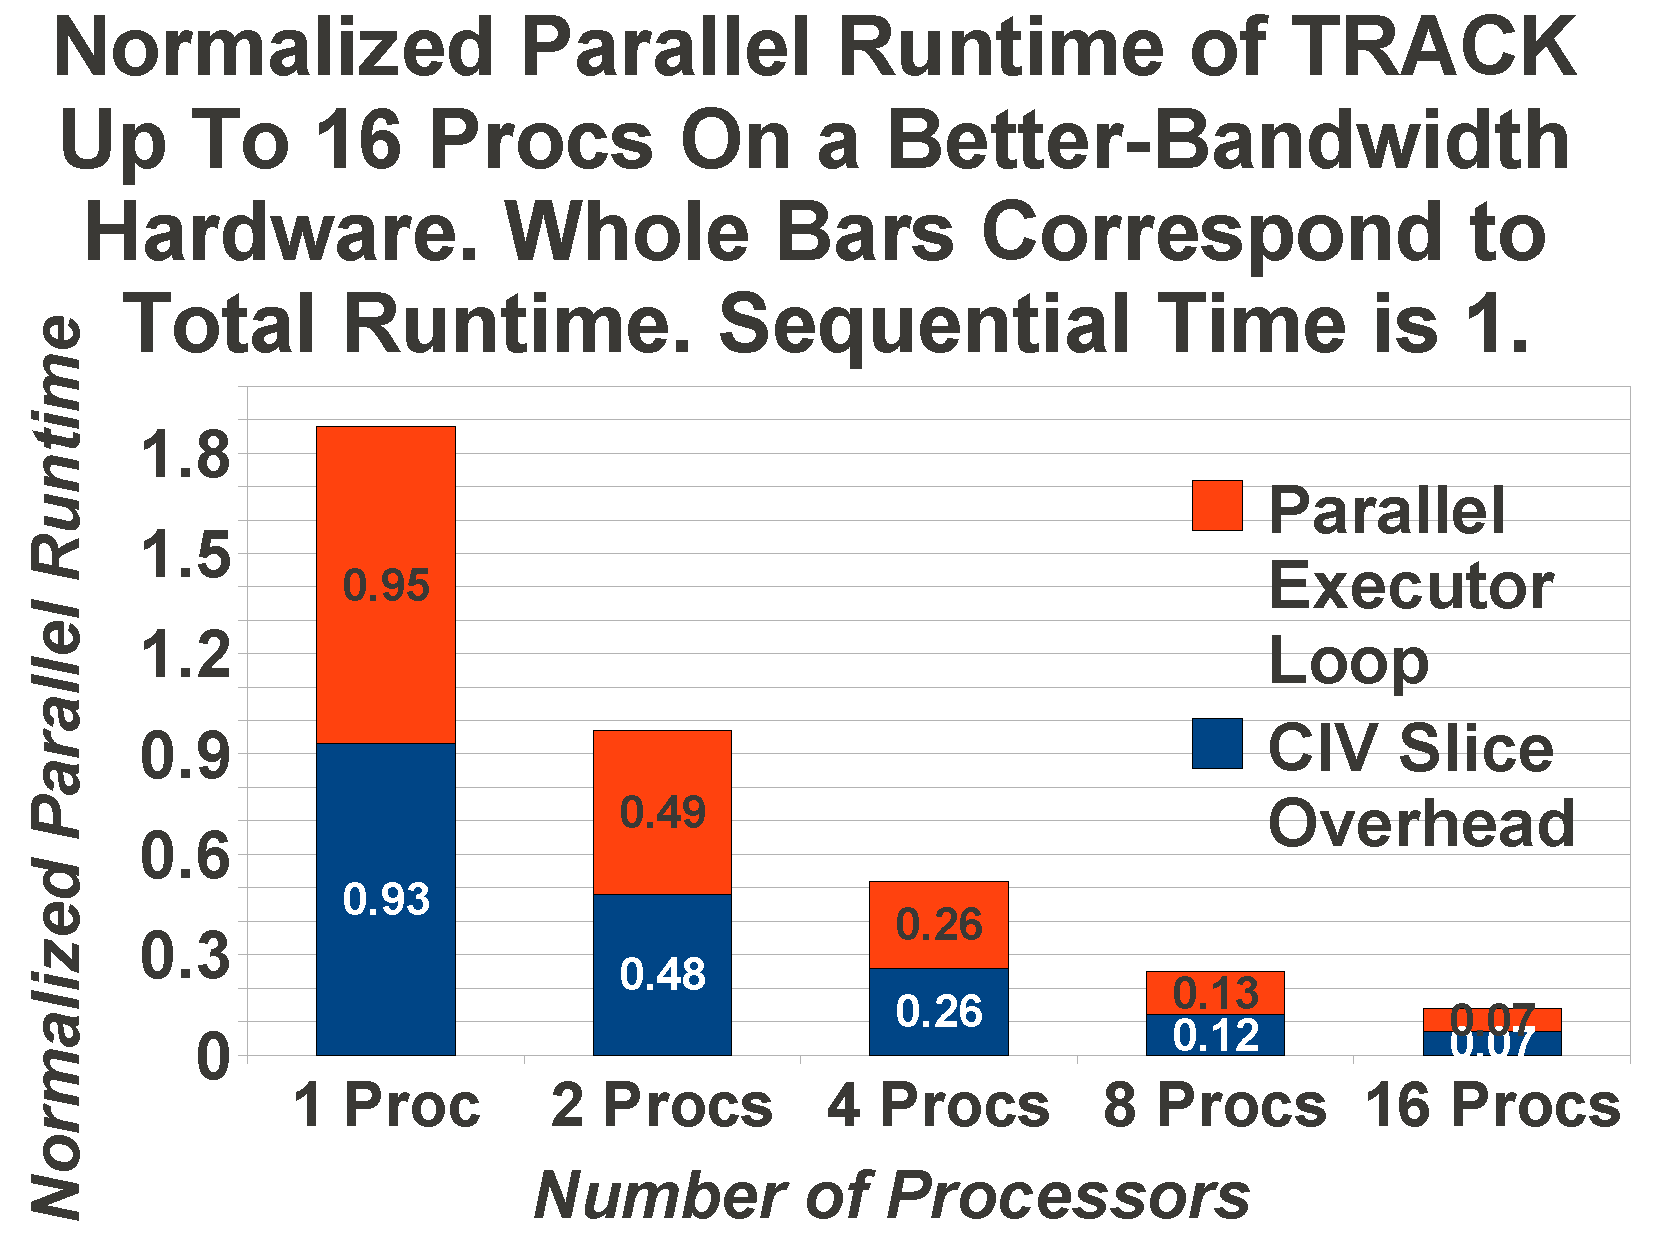
\includegraphics[width=.25\textwidth]{Figures/EmpRes/TrackScalNew}
%	}
%\end{tabular}
%\caption{ Benchmark and Loop-Level Normalized Runtime and Scalability Results. }
%\label{fig:ParRuntime} %
%\end{figure}



\vspace{1ex}


{\bf Experimental Methodology.} Our source-to-source compiler receives as
input a sequential {\tt Fortran77} program and automatically analysis loop-level 
parallelism and produces {\tt OpenMP} code.  The sequential and parallel 
code were compiled with {\tt gfortran}, option {\tt -O3}, and were run on 
a $16$-core {\tt AMD Opteron(TM) 6274} system with $128${\tt GB} memory. 
%Results were averaged for three independent runs.
%
%(-O4) and tested against IBM’s xlf compiler version
%13 on a 8 dual-core POWER 5+@1.9GHz, 32Gb-memory machine.

%\enlargethispage{\baselineskip}

\vspace{1ex}


{\bf Results} are depicted in Figure~\ref{fig:ParRuntime}. 
%
The top-left and top-right charts show the normalized-parallel runtime for each 
entire benchmark and {\sc civ} loop, respectively, where the {\sc civ}-computation
overhead is included in each bar.
%  where bars with names ending 
%in {\tt \_OV} show separately (only) the (non-negligible) runtime overhead of 
%(pre)computing the {\sc civ}s. 
%Note that the {\sc civ}-(pre)computation overhead is included
%for in the corresponding benchmark/loop bar.


Table~\ref{tab:LoopBenchProps} shows that the {\sc civ}-computation slice 
(i) represents a small fraction $6\%$ of the execution of the {\tt pric\_r}
benchmark,
%loop for {\tt PRICE\_R\_do10}, 
but (ii) it accounts for $45\%$ of the parallel execution time for {\tt track}.
The latter case is not surprising since the slice contains almost all statements 
of the original loop, i.e., {\tt EXTEND\_do400} and {\tt FPTRACK\_do300}, 
and both the loop and the slice are executed in parallel.    
Overall, for track we obtain a speedup of (only) $2.5$x on eight cores.


The less-than-optimal runtime for {\tt bdna}, {\tt nasa7}, and 
{\tt tree} was already explained, i.e., significant time spent in {\sc io},
small data sets. However, their loops show better results,
e.g., {\tt ACCEL\_do10} shows a  $7.1$x speedup on eight cores. % healthy

The loop-level scalability results of the bottom-left chart hint that 
memory bandwidth is the main limitation: 
For example, {\tt track}'s loops, overheads included, seem to scale well up to four cores,
not so well on eight, and poor on sixteen. %(and its overhead has a similar behavior).
The other-loops scalability is affected when passing from eight to sixteen
cores, e.g., {\tt ACCEL\_do10} shows (only) $11$x speedup on sixteen cores.
%, in comparison to $7.1$x on eight.

%(-O4) and tested against IBM’s xlf compiler version
%13 on a 8 dual-core POWER 5+@1.9GHz, 32Gb-memory machine.
To check this prediction we run {\sc track}, the most complex benchmark in our suite, 
on a bandwidth-friendlier system: an eight dual-core {\tt POWER 5+@1.9GHz} with $32$GB memory. 
The results, depicted in the bottom-right chart of Figure~\ref{fig:ParRuntime} show 
significantly-improved scalability up to sixteen cores for the total runtime. 
The {\sc civ}-computation overheads, also depicted in the chart, scale equally well.  
%and 
%the {\sc civ}-computation overhead of {\tt track}.
 
In summary, the benchmarks tested on four and eight processors show
an average speedup of $2.5$x and $5.13$x, and similarly 
the average speedup of loops is $2.86$x and $5.26$x, on four and eight cores, 
respectively.   The highest observed speedup, corresponding to {\tt price\_i}, 
is $12.5$x on sixteen cores.


\section{Related Work}
\label{sec:RelWork}

Classical loop analysis examines each pair of read/write accesses, % dependence each
and models dependencies into linear systems of (in)equations that are solved
statically  via Gaussian-like elimination~\cite{BanerjeeIneqTest,FeautrierDataflow}. %Pugh92theomega
Such analysis  can drive powerful code transformations to optimize 
parallelism~\cite{PolyhedralOpt}, albeit in the narrow(er) domain 
in which subscripts, loop bounds, {\tt if} conditions are affine 
expressions of loop indices.

Several techniques have been proposed to handle irregular subscripts that have
the shape of closed-form formulas in the loop indices. For example, 
The Range Test~\cite{Blume94RangeTest} uses symbolic 
ranges to disambiguate a class of quadratic and  
exponential subscripts by exploiting the monotonicity of the read-write pair 
of subscripts.   A class of indirect-array subscripts is solved with 
an idiom-recognition method~\cite{PaduaDemDrInterproc}, where interprocedural 
analysis verifies the (assumed) monotonicity of the values stored in the 
index array.
%
Furthermore, Presburger arithmetic was extended to support
uninterpreted functions~\cite{Pugh98NonlinPresb}, and the irreducible-result
formula is executed at runtime to disambiguate a class of irregular
accesses. 

A different type of approach, which was found more effective in
solving larger loops, is to encode loop independence into one equation 
on abstract sets, for each array. The abstract set models the
memory references of the corresponding array and is computed 
via interprocedural summarization of 
accesses~\cite{SUIF,Moon99PredArrDataFlow,SummaryMonot,LMAD}.
While each of these methods covers some irregular accesses,
none of them handles {\sc civ}-subscripted loops,   
such as the ones analyzed in this paper.
%

A related  body of work presents (i) symbolic-algebra systems that, for example,  
compute upper and lower bounds of nonlinear expressions~\cite{Fahringer97EffSymb},
and (ii) techniques to characterizes scalar-value monotonicity within a 
loop~\cite{VEG,MonStmt}.
%, and (iii) generalized formulations of induction variables~\cite{Engelen04aunified}.

This solves only half of the problem, which   
corresponds to establishing the monotonic properties of {\sc civ}s.
This paper addresses the second challenge: 
how to build array summaries by using the {\sc civ}-related invariants,
where the immediate application is verifying loop independence. 
Related solutions analyze special cases of accesses:
%
For example, a pair of accesses of form  
\begin{small}{\tt\{X(CIV),X(CIV+d)\}}\end{small}, where {\tt d} is a constant,
can be disambiguated by reasoning in terms of the
(range of the) cross-iteration evolution of the corresponding {\sc civ}~\cite{CohenBeyondMon}.
%
However, this does not address the case when a subscripts is affine
and the other uses {\sc civ}s, i.e., it might prove output 
independence for Figure~\ref{fig:codeActforCorrec}(b),
but will not prove flow independence for the loops in 
Figure~\ref{fig:codeActforCorrec} %~\ref{fig:Tree}(a)
or for {\sc track}. % for the loops of {\tt track} benchmark.

Enhancing the idiom-recognition support~\cite{PaduaStackArr,PaduaDemDrInterproc} 
allows to relate better the {\sc civ} properties with the dependency test: 
For example, in the loop in Figure~\ref{fig:codeActforCorrec}(a), the write to 
{\tt X(civ)} matches the pattern of a consecutively-written single-index ({\sc cw-si}) 
array, and always covers the read from {\tt X(j)}, hence array {\tt X} is privatizable,
and the stack access in Figure~\ref{fig:Tree}(a) falls into a similar pattern.
%
%
However, loops such as the one in Figure~\ref{fig:codeActforCorrec}(b),
or {\sc track}, are unanalyzable because 
the subscripts are neither single indexed, nor consecutively written.  

In comparison, over/under-estimate summarization allows us,
intuitively, to reduce the problem to a known idiom, albeit
the code does not fall, strictly speaking, within that idiom.
Furthermore, other than {\sc veg}, our analysis does not rely
on pattern matching, but discovers non-trivial invariants that
enable the {\sc civ}-agnostic test either (i) to prove loop independence,
%e.g., Figure~\ref{fig:codeActforCorrec}(b), 
or (ii) to be tuned in a manner that resolves a specific pattern 
of dependencies, e.g., {\sc track}.

Finally, the value-evolution graph has been applied in the context of 
autoparallelization~\cite{VEG}.   The high-level difference is that there, 
subscripts are separated early into {\sc civ}-based and affine and they 
do not mix: they are summarized under different representations, 
and disambiguated via specialized dependency tests.
Analysis builds only accurate summaries, which may restrict the
effectiveness of dependency tests. 
%are identified through a {\sc cw-si}-like heuristic.
More specifically, there are not reported:
  (i)   symbolic, non-constant {\sc civ} evolutions,
        e.g., Fig~\ref{fig:codeActforCorrec}(b),
 (ii) the complex output-dependency pattern of {\sc track},
(iii) extraction of runtime predicates for {\sc civ}-dependence tests,
 (iv) prefix-sum precomputation of {\sc civ} values, in the
        cases when they are used as data, rather than for indexing,
  (v) privatization of stack-like accesses, 
 (vi) runtime and scalability results.

%%%%%%%%%%%%%%%%%%%%%%%%%%%%%%%%

\section{Conclusions}
\label{sec:Concl}

This paper has presented an analysis that summarizes both 
affine and {\sc civ}-based subscripts under the same 
representation. 
%
%We have shown how the
%result summaries are used by {\sc civ}-agnostic dependency
%tests, but their application is wider, e.g., array {\sc ssa}. 
%
%This paper has presented a flow-sensitive summarization analysis that 
%verifies the symbolic invariants which allow {\sc civ}-based
%subscripts to be handled similarly to affine ones. 
%
The result summaries are {\sc civ} agnostic and can be used for 
various  purposes, e.g., dependence analysis or array {\sc ssa}. 
%
Our analysis seems less conservative than related approaches 
in that the algebra of under/over-estimates can exploit partial 
programming idioms, such as vectors in which elements are mostly 
pushed but some are overwritten. %or the vectors with holes.

We have reported an automatic solution that is well integrated 
in the repertoire of a compiler that combines static and dynamic 
techniques to aggressively parallelize loops, and have 
demonstrated the viability of the approach via a systematic
evaluation of five real-world applications.

%\bibliographystyle{abbrvnat}
\bibliographystyle{abbrv}
%\softraggedright
\begin{small}
\bibliography{CIVpaper}
\end{small}

\newpage

\section{Appendix: Beyond Monotonicity} % : Privatizing Stack-Like Accesses
\label{sec:Stack}

While we have studied so far the case when the {\sc civ} evolution
throughout a loop is monotonic, this Section investigates a stack-like 
access pattern that can still be solved in a similar fashion, by 
studying monotonicity piecewise.
 
For example, the code in Figure~\ref{fig:Tree}(a) is a simplified
version of loop {\tt ACCEL\_do10} from {\tt tree} benchmark. 
The logic is that each iteration of the outer loop maintains its own
stack, denoted {\tt X}, that is used in the {\tt while} loop to 
compute a result {\tt res}:
The {\tt while} loop is exited when the stack is empty, and each
iteration pops one element and, later on, pushes
up-to-eight new elements from/to the stack. 

The goal is to prove that the stack {\tt X} is privatizable in the
context of the outer loop.   The plan is to devise an analysis
capable of overestimating, via {\em disjoint intervals}, the   % i.e., strided intervals.
{\tt while}-loop-aggregated (i) {\em read set}, i.e., 
{\sc r} $=$ {\sc ro} $\cup$ {\sc rw}, and (ii) {\em write-first set}. 
In our case, this would result in  
$\lceil${\sc r}$\rceil=${\tt[0,civ-1]}, and
$\lceil${\sc wf}$\rceil=${\tt[civ,SS]}, where {\tt SS} denotes
the stack size and  {\tt civ} is the value before entering the 
{\tt while} loop, i.e., $1$.  

One can now observe that the read set of the {\tt while} loop 
is included in the {\sc wf} set of the region just before the 
{\tt while} loop, i.e., {\tt \{0\} $\subseteq$ \{0\}}, due to the 
first update to {\tt X(civ)}. It follows that the read set of
each iteration of the outer loop is the empty set, 
hence {\tt X} can be safely privatized. 


\begin{figure}
\begin{minipage}{0.4\columnwidth}
\begin{colorcode}
DO i = 1, N, 1
 civ = 1
 {\bf{}X}(civ) = ...
 WHILE ( civ .GT. 0 )
  civ@2 = \mymath{\gamma}(civ,civ@5)
  q = {\bf X}(civ@2)
  civ@3 = civ@2 - 1
  IF (q .LE. 5) THEN
   res = res + .. q ..
  ELSE
   DO j = 1, 8, 1
    IF (civ .LT. SIZE) 
      civ = civ + 1
      {\bf{}X}(civ) = ...
   ENDIF ENDDO
   civ@9 = \mymath{\gamma}(civ@3,..)
  ENDIF
  civ@5=\mymath{\gamma}(civ@3,civ@9)
ENDWHILE ENDDO   
\end{colorcode}
\vspace{-1ex}
(a) Loop {\tt ACCEL\_do10}.
\end{minipage}
\begin{minipage}{0.56\columnwidth}
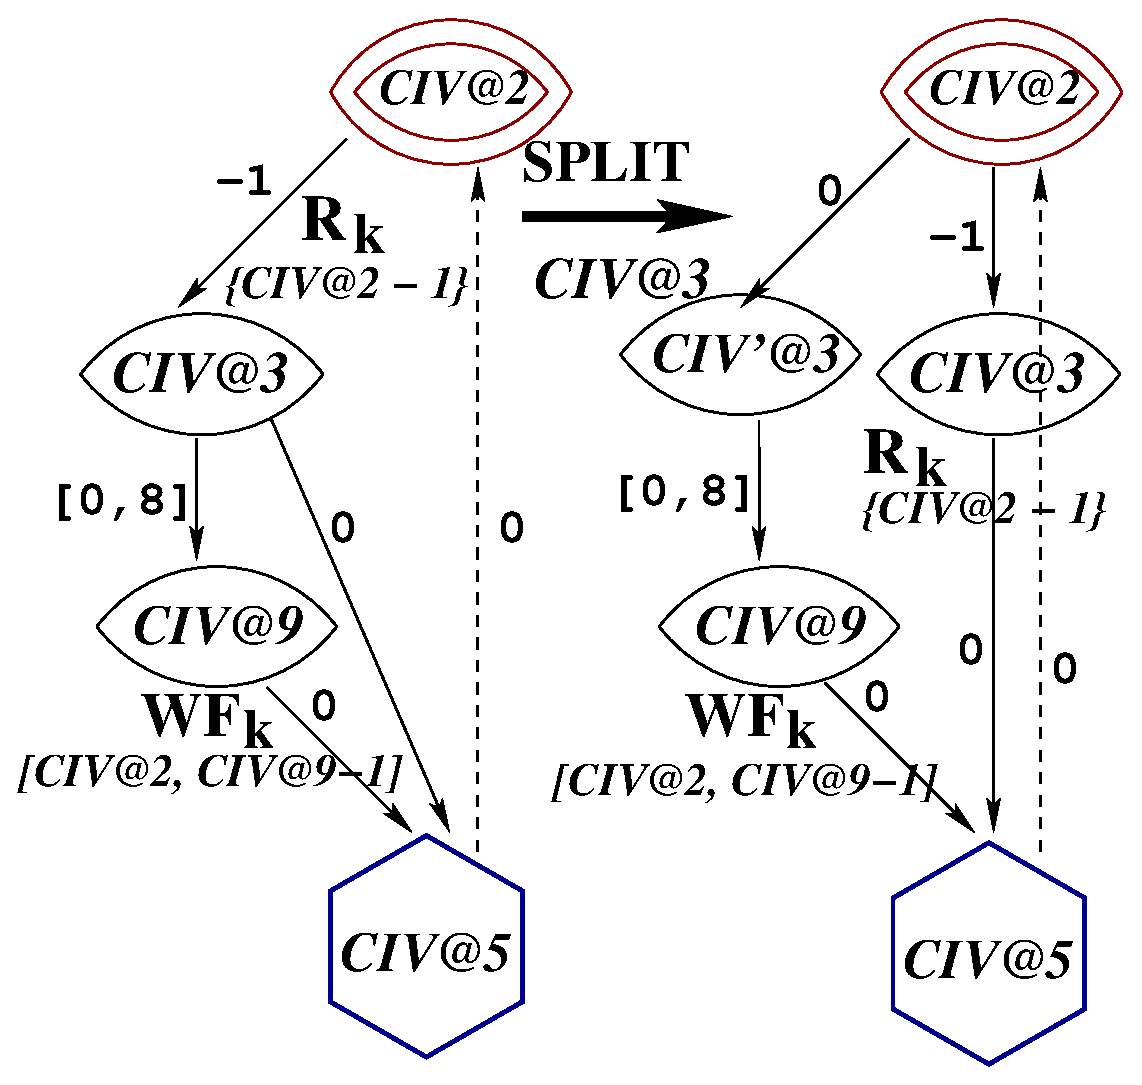
\includegraphics[width=1.1\textwidth]{Figures/VEG_TREE}\\
(b) Original \& Transformed {\sc veg}s.
\end{minipage}
\hrule
\caption{a) Stack-like access in benchmark {\tt tree} and (b) the {\sc veg} graphs of the while loop.}
\vspace{-1ex}
\label{fig:Tree} %
\end{figure}


The original {\sc veg} of the {\tt while} loop, depicted on the left 
side of Figure~\ref{fig:Tree}(b), exhibits a non-monotonic {\sc civ}$_\mu$
evolution, i.e., it can be anywhere between minus one and seven.
%
The intuition is to use an inductive summarization for the read and {\sc wf} sets:
{\em The base case} corresponds to analyzing the first iteration to determine a split point, 
denoted {\tt SP}, from which, without loss of generality, the write-first set increases in the 
upper-bound direction, i.e., {\sc wf}$=${\tt[SP, ...]$^s$}, and the read set increases in the lower-bound
direction, i.e., \\
{\sc r}$=${\tt [..., SP-$s$]$^s$}, where $s$ denotes the interval stride.
(The other case is treated in a similar fashion).

With our example, {\sc wf}$_k=${\tt (q.GT.5)\#[civ@2,civ@9-1]}
is associated with {\sc veg} node {\tt civ@9}, and 
{\sc r}$_k=${\tt \{civ@2-1\}}, as before, with {\tt civ@3}, 
where $k$ denotes an arbitrary iteration of the {\tt while} loop.
The split point is {\tt SP=civ=1}, since {\tt civ@2} equals {\tt civ} 
for the first iteration.


%With our example, {\sc r}$_k=${\tt \{civ@2-1\}} is associated, as before, with
%{\sc veg}-node {\tt civ@3}, and \\
%{\sc wf}$_k=${\tt (q.GT.5)\#[civ@2,civ@9-1]}
%with node {\tt civ@9}, where $k$ denotes an arbitrary iteration of the {\tt while} loop.
%The split point is {\tt SP=civ=1}, since {\tt civ@2} equals {\tt civ} 
%for the first iteration.

{\em The second step} is to attempt a semantics-preserving {\sc veg} transformation
such that (i) each {\sc civ}-decreasing/increasing path holds only intervals 
belonging to the read/{\sc wf} set, respectively, and (ii) a $0$-path holds
only empty intervals.

The semantics to be preserved is that the aggregated-read/{\sc wf} summaries of
any valid execution of the original {\sc veg} should be preserved by (at least) one 
valid execution of the transformed {\sc veg}.  The approach is
to search for a path where, say, the read set occurs before a {\sc wf} set.
One can then split/clone a convenient node {\sc civ}$_{sp}$ between the two, and 
introduce a $0$-evolution path from {\sc civ}$_{sp}$ to the back node, if none already exist,
and a $0$-evolution path from {\sc civ}$_\mu$ to the cloned-node {\sc civ}$_{sp}^{cl}$.
The original path is translated with the original path up to {\sc civ}$_{sp}$,
then directly to the back node, followed by the $0$-evolution path to  
{\sc civ}$_{sp}^{cl}$, and the rest of the original path. The splitting can be
repeated to a fix-point.

For example, the right side of Figure~\ref{fig:Tree}(b) shows the result of
splitting  node {\tt civ@3} of the original {\sc veg}: a new $0$-evolution
edge now connects {\tt civ@2} and {\tt civ'@3}. In addition, the {\sc wf} set 
has been adjusted to the new {\sc civ}$_\mu$ value, but has also
been conservatively extended with the result of the read-set of the previous
(transformed) iteration, resulting in the same $WF_k$ interval as 
in the original {\sc veg}. 



{\em Finally, the third step} is to aggregate the {\sc wf} and read sets 
only on the monotonically increasing and decreasing (including $0$) paths,
respectively. 
If the read and {\sc wf} results are exact, i.e., the under 
and overestimate are identical, and have shapes {\tt [..., SP-$s$]$^s$}  
and {\tt[SP, ...]$^s$}, respectively, then 
one can prove that the result of this piecewise monotonic
aggregation matches the result of the original-{\tt while} aggregation:
an overestimate of the 
%{\tt while}-aggregated 
read set is {\tt [0,SP-$s$]$^s$}, i.e., 
we have achieved our goal. 
%and analysis continues as described in the beginning of this section. 
Note that the lower bound can be improved by using the {\tt while}-stop condition. 
The formalization of this step is presented in Appendix~\ref{app:TheoremProof}. 
%necessary

\section{Appendix: Theorem Proof} %in Section~\ref{sec:Stack}
\label{app:TheoremProof}

\newdef{definition}{WF$_{pred}$/R$_{pred}$}
\begin{definition}
We denote by {\tt UB$_j$} and {\tt LB$_j$} the upper and lower bounds corresponding
to the monotonic aggregation of the {\sc wf} and {\sc read} sets of some iteration
$j$ in the transformed {\sc veg}, where both {\tt UB$_j$} and {\tt LB$_j$} are
affine function of the {\sc civ}$_\mu$ of iteration $j+1$.
We {\bf define} $WF_{pred}^{i} = ${\tt[SP, MAX$_{j=1}^{i}$(UB$_j$)]$^s$} and, similarly, 
$R_{pred}^{i} = ${\tt[MIN$_{j=1}^{i}$(LB$_j$), SP$-s$]$^s$}, where $s$ is the stride,
and {\tt MAX$_{j=1}^{i}$(UB$_j$)} denotes the maximal-encountered upper bound in the
(non-monotonic) execution of iterations $1 .. i$ of the transformed {\sc veg},
and similarly for {\tt MIN$_{j=1}^{i}$(LB$_j$)}.
\end{definition}

\newtheorem{theorem}{CIV Piecewise Monotonicity}
\begin{theorem}
{\bf If} the read and {\sc wf} sets appear only on monotonically increasing and decreasing 
{\sc veg} paths, respectively, and they can be exactly aggregated  when considering only the
corresponding monotonic paths, and furthermore they correspond to disjoint intervals ({\sc lmad}s), 
whose union is contiguous,
{\bf then} $R^i = R_{pred}^{i}$ and $WF^i = WF_{pred}^{i}$, where $R^i$ and $WF^i$
denote the loop-aggregated read and {\sc wf} result of iterations $1..i$,
as defined, for example, in Figure~\ref{fig:LoopAggreg}.
\begin{proof}
The proof is by induction after $i$. %\vspace{1ex} 

I. The base case is verified by construction, i.e., it was already checked that the 
read and {\sc wf} set of iteration $1$ have shape 
{\sc r}$=${\tt [...,SP-$s$]$^s$} and {\sc wf}$=${\tt[SP,...]$^s$}, which are exactly
$R_{pred}^i$ and $WF_{pred}^{i}$. \vspace{1ex}  

II. We assume that $R^1 = R_{pred}^{1}$, ..., $R^{i-1} = R_{pred}^{i-1}$ hold, and we
prove that $R^i = R_{pred}^{i}$ (the {\sc wf} case is treated similarly). \vspace{1ex}  

II.1 If iteration $i$ has increasing or $0$ evolution than its read set is empty, hence
$R^i=R^{i-1}$ and $R_{pred}^{i-1} = R_{pred}^i$ and by induction hypothesis 
$R^{i-1}=R_{pred}^{i-1}$. It follows that $R^i = R_{pred}^{i}$. \vspace{1ex}  

II.2 Consider iteration $i$ has increasing evolution. We take $e \in R_{pred}^{i} - R_{pred}^{i-1}$
and prove that $e \in R^{i}$, i.e., $R_{pred}^{i} \subseteq R^i$. 
Note that if $e \in R_{pred}^{i-1}$ then by induction hypothesis
$e \in R^{i-1}$ which implies $e \in R^{i}$ since $R^{i-1} \subseteq R^i$  
(also $R_{pred}^{i-1} \subseteq R_{pred}^{i}$, i.e., monotonically increasing sequences). \vspace{1ex}

II.2.a If by absurd, $e \ge {\tt{}SP}$ then there has been a previous {\sc civ}-increasing 
iteration $i'$ such that $e \in WF_{pred}^{i'}$. By induction hypothesis $e \in WF^{i'}$, 
hence $e$ cannot be the contribution of iteration $i$ to the
loop-aggregated read set, contradiction. \vspace{1ex}

II.2.b If {\tt{}MIN$_{j=1}^{i-1}$(LB$_j$)}$ \le e < {\tt{}SP}$, then, 
there must have been a previous {\sc civ}-decreasing iteration $i'$ that has
reached a lower-bound smaller than $e$, and since $R_{pred}^{i'}$ is contiguous
modulo the stride, then $e \in R_{pred}^{i'} = R^{i'} \subseteq R^{i}$.  \vspace{1ex}

II.2.b Finally, case {\tt{}MIN$_{j=1}^{i}$(LB$_j$)}$\le e < ${\tt{}MIN$_{j=1}^{i-1}$(LB$_j$)}
implies that iteration $i$ is the first to reach a lower bound less-or-equal to $e$.
Since, by hypothesis, the per-iteration read set is exactly described, then $e$ must 
be read in iteration $i$. It follows that either $e \in WF^{i-1}=WF^{i}$
or $e \in R^i$. However, $e \not\in WF^{i-1}$ since the current iteration is the first one
to go beyond {\tt{}MIN$_{j=1}^{i-1}$(LB$_j$)}.  Hence, $e \in R^i$. 
%Since iteration $i$ $WF^{i-1}$ 
%is the first one to reach $e$ then $e$ cannot belong to $WF^i$, hence it necessarily
%belongs to $R^i$.  
\vspace{1ex}

II.3 Consider iteration $i$ has increasing evolution. We take $e \in R^{i} - R^{i-1}$
and prove that $e \in R_{pred}^{i}$, i.e., $R^i \subseteq R_{pred}^{i} $. 
The proof is similar to $R_{pred}^{i} \subseteq R^i$.
\end{proof}
\end{theorem}

\end{document}


%%%%%%%%%%%%%%%%%%%%%%%%%
%%%% USELESS STUFF %%%%%%
%%%%%%%%%%%%%%%%%%%%%%%%%

